\documentclass{article}
\usepackage{graphicx} % Required for inserting images
\usepackage{amsmath}    % \begin{equation}, \eqref, \lVert, \Bigl, …
\usepackage{amssymb}    % math symbols
\usepackage{microtype}  % better kerning, optional
\usepackage{hyperref}   % clickable refs (keep last)
\usepackage[T1]{fontenc}          % modern fonts, fixes UTF-8 dashes
\usepackage{lmodern}              % Latin Modern font
\usepackage[square,comma]{natbib} % enables \citep and \citet
\usepackage{float}
\usepackage[dvipsnames]{xcolor}

\title{A Minimal Disformal Scalar Framework for Emergent Geometry and Stress–Energy}
\author{Moeidh Mana Hanash}
\date{August 2025}

\begin{document}

\maketitle
\begin{abstract}
We develop a minimal one-field framework in which a real scalar $\Phi$ defines both the effective spacetime geometry and its associated stress–energy. The construction is a rank-one Bekenstein-type disformal transformation of Minkowski,
\begin{equation}
S=\int d^4x\Big[-\tfrac{1}{2}(\partial\Phi)^2 - V(\Phi) - \tfrac{\alpha}{4}(\partial\Phi)^4\Big],
\qquad
g^{\rm eff}_{\mu\nu}=\eta_{\mu\nu}+\alpha\,\partial_\mu\Phi\,\partial_\nu\Phi, \label{1}
\end{equation}
with closed-form inverse and determinant from Sherman–Morrison identities. The field equation is quasilinear, strictly second order, and hyperbolic for $1+\alpha X>0$ with $X=\eta^{\mu\nu}\partial_\mu\Phi\,\partial_\nu\Phi$. The quartic gradient acts as a Skyrme-like stabilizer: a covariant virial identity yields $E_{\mathcal G}=\mathcal T+3V$, showing that finite-energy stationary solitons are compatible with Derrick’s theorem in $3{+}1$ dimensions. The energy functional is coercive and bounded below for $\alpha>0$ and $V\!\ge\!0$, and 1-D kink-type numerics confirm stable minima and scaling relations.

\emph{Scope of Part I.} We assume universal minimal coupling of all matter (including electromagnetism) to $g^{\rm eff}_{\mu\nu}$, so rods, clocks, and photons follow the effective metric. Restricting to the \emph{conservative weak-field sector through second post-Newtonian order}, we find the Parametrized Post-Newtonian values $\gamma=\beta=1$ with no preferred-frame effects, and we recover GR light-deflection and Shapiro delay. Dissipative dynamics (radiation reaction, waveform phasing), higher-order PN effects, and strong-field phenomenology are deferred to Parts II–III of the trilogy.
\end{abstract}

\section{Introduction}

General relativity (GR) represents one of the central conceptual advances of modern physics \cite{Einstein1916_GR}. In Einstein’s framework, spacetime is promoted from a passive stage to a dynamical entity whose curvature governs the motion of matter and light. The Einstein field equations equate geometry, expressed through the Einstein tensor, with the stress--energy tensor $T_{\mu\nu}$ that encodes the distribution of matter and radiation. While this synthesis elegantly unifies inertia and gravitation at the level of trajectories, it retains an asymmetry at the level of ontology: the metric $g_{\mu\nu}$ evolves dynamically, but $T_{\mu\nu}$ is introduced phenomenologically from external matter models \cite{Will2014_LivingRev}. Spacetime and matter thus remain conceptually distinct, coupled but not derived from a common origin. Observationally, the equivalence principle indicates a deep unity between inertia and gravitation, yet in GR this unity is imposed rather than derived: inertial properties follow from postulated matter fields, while gravitation follows from curvature. A framework in which both curvature and stress--energy arise from a single underlying degree of freedom would provide a more economical description and potentially explain the proportionality of inertial and gravitational mass as a dynamical consequence rather than as an axiom.

Efforts to realize such unification have taken several forms over the past century. Scalar--tensor theories, most prominently the Brans--Dicke model \cite{Brans1961}, sought to make Newton’s constant dynamical by introducing an additional scalar degree of freedom embodying Mach’s principle. Higher-dimensional proposals, beginning with Kaluza’s unification of gravity and electromagnetism \cite{Kaluza1921} and Klein’s quantum reinterpretation \cite{Klein1926}, embedded four-dimensional spacetime in a larger manifold so that gauge fields arise as components of a higher-dimensional metric. Nonlinear extensions of the gravitational action, including Born--Infeld–type constructions inspired by Eddington’s affine approach \cite{Banados2010_EiBI}, modified the high-curvature regime while reproducing GR at low energies. Each of these directions offered partial progress toward blending matter and geometry, but all required either multiple dynamical fields, extra dimensions, or nontrivial modifications of the Einstein–Hilbert action.

The Proto–Field Gravity Model (PFGM) follows a more radical route. It postulates that a single real scalar field $\Phi$ constitutes the sole dynamical degree of freedom, responsible both for generating effective spacetime geometry and for producing the stress–energy conventionally attributed to matter. In this construction, the effective metric is not introduced ad hoc but arises algebraically from gradients of $\Phi$ through a rank-one disformal transformation of the Minkowski background \cite{Bekenstein1993,Bettoni2013}. This structure ensures that the resulting equations of motion remain quasilinear and second order, thereby avoiding higher-derivative pathologies associated with Ostrogradsky instabilities \cite{Woodard2015}. No additional propagating degrees of freedom are introduced, making PFGM a minimalist yet internally consistent attempt at a one-field unification of matter and geometry.

Several considerations motivate this one–field ontology. From a classical perspective, general relativity predicts singularities at extreme densities, reflecting the separation between geometry and sources. In PFGM, this division is absent: the same scalar gradients that generate stress–energy also determine the effective metric, introducing a natural feedback mechanism that can regulate high-density configurations. The theory is consistently defined within the hyperbolic domain
\begin{equation}
1+\alpha X > 0, 
\qquad 
X \equiv \eta^{\mu\nu}\partial_\mu \Phi \,\partial_\nu \Phi ,\label{2}
\end{equation}
where the Cauchy problem is well posed and the characteristics coincide with the null cones of the disformal metric \cite{Bekenstein1993,Bettoni2013}. This condition guarantees a consistent causal structure and permits stability analyses within a mathematically controlled regime.

Cosmology provides a complementary motivation. Observational constraints, most prominently the Planck 2018 results \cite{Planck2018_Cosmology}, indicate that the cosmic energy budget is dominated by dark matter and dark energy, whose physical origin remains uncertain. If a single scalar field $\Phi$ underlies both the effective spacetime geometry and the associated stress–energy, then at least part of the phenomenology attributed to dark components may be reformulated within a more economical framework. Although explicit cosmological solutions are not developed in this first analysis, the potential relevance of PFGM to large–scale dynamics motivates treating it as a candidate framework for unification.

Quantum field–theoretic considerations suggest further advantages. If the vacuum expectation value of $\Phi$ defines the effective metric, then radiative corrections acquire a direct geometric interpretation. Within the effective field theory window set by the strong–coupling scale $\Lambda_\alpha=\alpha^{-1/4}$, destabilizing higher-dimension operators are naturally suppressed and no higher-derivative ghosts are introduced \cite{Burgess2007_EFT}. The consistency of the construction follows directly from the algebraic form of the disformal transformation, without appeal to hidden symmetries or fine-tuned cancellations. These features strengthen the case for PFGM as a conservative but conceptually novel framework in which matter and geometry are unified.

The formulation is deliberately minimal. A single scalar $\Phi$ fulfills three roles simultaneously: it defines the rods and clocks of measurement, it generates the effective stress–energy, and it produces the curvature of the emergent metric. Localized configurations of $\Phi$ appear as finite–energy solitons, with gradients directly shaping spacetime geometry. A central ingredient is the quartic gradient term in the energy functional, proportional to $\alpha (\partial \Phi)^4$, which acts as an internal pressure. This term modifies scaling behaviour: once the virial balance is imposed, the energy functional develops a nontrivial minimum at finite size. In this way PFGM circumvents Derrick’s theorem in flat space \cite{Derrick1964} while maintaining strictly second–order dynamics.

The stabilizing mechanism is directly analogous to the Skyrme term in nuclear soliton models, where quartic derivative interactions were introduced to overcome the same scaling obstruction and to generate finite-size baryonic solitons \cite{Skyrme1961,Adkins1983}. The analogy emphasizes the conservative character of the construction: stability is achieved without additional fields or exotic operators, but rather through the algebraic structure of the emergent metric.

By contrast, earlier attempts to construct purely scalar models of gravity encountered two canonical obstacles. The first is Derrick’s theorem, which states that in three spatial dimensions static scalar configurations supported only by a canonical kinetic term $(\partial \Phi)^2$ and a potential $V(\Phi)$ are unstable under scale transformations. Under the rescaling $\Phi(x)\to\Phi(\lambda x)$, the kinetic energy scales as $\lambda^2$ and the potential as $\lambda^3$, so the total energy $E(\lambda)$ has no stationary point at finite $\lambda$. Any putative soliton therefore dilates without bound or collapses to zero size \cite{Derrick1964}. Classical stability appeared unattainable unless supplemented by additional structures such as gauge interactions, higher–order spatial gradients, or nontrivial topology.  

The second obstacle is the appearance of Ostrogradsky instabilities in higher–derivative scalar theories. In PFGM, the quartic correction arises algebraically from the disformal structure rather than from higher time derivatives. The field equations remain quasilinear and strictly second order, thereby avoiding the Hamiltonian instabilities guaranteed by Ostrogradsky’s theorem \cite{Woodard2015}. In this respect, the stabilizing mechanism is conceptually analogous to the Skyrme term in nuclear physics \cite{Skyrme1961,Adkins1983}, but here it is implemented through a minimal disformal update of the metric. The theory thus retains a single propagating scalar degree of freedom while remaining free of ghosts.  

These features place PFGM within the broader landscape of scalar–tensor and modified gravity frameworks. Traditional scalar–tensor theories such as Brans–Dicke \cite{Brans1961}, their generalization to Horndeski’s second–order class \cite{Horndeski1974}, and later Galileon extensions \cite{Nicolis2009_Galileon,Deffayet2011_Galileon} all introduced new operators to stabilize scalar dynamics while preserving second–order equations. Mimetic constructions \cite{Chamseddine2013_Mimetic} and Born–Infeld–inspired theories \cite{Banados2010_EiBI} pursued alternative nonlinear completions. Comprehensive reviews are available in \cite{Clifton2012,Joyce2015,deRham2014_Review}. PFGM differs in that it neither enlarges the field content nor invokes hidden symmetries, but instead derives its stabilizer directly from the geometry defined by $\partial_\mu\Phi$. As will be shown in the sections that follow, this minimal structure suffices to evade Derrick’s theorem, avoid Ostrogradsky instabilities, and provide a basis for effective field theory and cosmological applications \cite{Mukhanov2005}.

This article (Part~I of a trilogy) is restricted to the \emph{foundational and conservative weak-field sector through second post-Newtonian (2PN) order}. We assume universal minimal coupling of all matter (including electromagnetism) to the emergent metric \(g^{\rm eff}_{\mu\nu}\), so rods, clocks, and photons follow \(g^{\rm eff}_{\mu\nu}\). Within the well-posedness domain (hyperbolicity \(1+\alpha X>0\) and stability \(P_X>0\), \(P_X{+}2X P_{XX}>0\)), we establish that the conservative PPN parameters match GR through 2PN (in particular \(\gamma=\beta=1\) with no preferred-frame effects) and that light-deflection and Shapiro delay agree with GR. \emph{Radiative dynamics, waveform phasing, and higher-order PN effects (3PN/4PN) are \textbf{not} treated here and are deferred to Part~II; strong-field structure and echo phenomenology are deferred to Part~III.}

%%%%%%%%%%%%%%%%%%%%%%%%%%%%%%%%%%%%%%%%%%%%%%%%%%%%%%%%%%%%%%%%

\section{Minimal action, field equations, and emergent metric}
\label{sec:action}

The foundation of the Proto–Field Gravity Model (PFGM) is a single real scalar field endowed with a quartic derivative interaction that simultaneously determines spacetime geometry and stress–energy. This section introduces the minimal Lorentz-invariant action, the emergent disformal metric, and the resulting field equations, formulated within a rigorously well-posed effective field theory (EFT) framework.

\subsection{Postulates and notation}

We adopt the following conventions. Spacetime is the smooth manifold $\mathbb{R}^{1,3}$ with Minkowski metric $\eta_{\mu\nu}=\mathrm{diag}(-1,+1,+1,+1)$, and indices are raised and lowered with $\eta_{\mu\nu}$ unless otherwise specified. Greek indices $\mu,\nu,\dots$ run over $0,1,2,3$, and Latin indices $i,j,\dots$ denote spatial components. Einstein summation is assumed. Partial derivatives are denoted by commas, e.g. $\Phi_{,\mu}\equiv\partial_\mu\Phi$. In flat space, $\nabla_\mu\Phi=\partial_\mu\Phi$, and the d’Alembertian is $\square\equiv\eta^{\mu\nu}\partial_\mu\partial_\nu$. Natural units ($\hbar=c=1$) are used, so length, time, and mass have dimensions of inverse energy. Newton’s constant $G_N$ is kept explicit, with reduced Planck mass $M_{\rm Pl}^2=(8\pi G_N)^{-1}$.
\paragraph{Conventions.}
We use signature $(-,+,+,+)$ and define
\[
X \;\equiv\; \eta^{\mu\nu}\,\partial_\mu\Phi\,\partial_\nu\Phi,
\qquad [\alpha]={\rm mass}^{-4},\qquad M_\alpha \equiv \alpha^{-1/4}.
\]
The field $\Phi$ has canonical mass dimension one. Unless stated otherwise, indices are raised/lowered with $\eta_{\mu\nu}$.

The dynamical variable is a real scalar field $\Phi(x)$ of canonical mass dimension one. Its self-interaction potential $V(\Phi)$ admits a nondegenerate vacuum at $\Phi_\infty$, with $V''(\Phi_\infty)>0$ to exclude tachyonic modes. A positive constant $\alpha$ of mass dimension $-4$ controls the quartic derivative interaction and defines the EFT cutoff scale $\Lambda_\alpha=\alpha^{-1/4}$ \cite{Burgess2020_EFTbook}. The parameter $\alpha$ sets the scale at which disformal corrections become relevant, and its value will later be constrained by Solar-System tests in analogy with disformal scalar–tensor theories subject to post-Newtonian bounds \cite{Ip2015_DisformalPPN}.

The resulting field equations are quasilinear and strictly second order, ensuring well-posedness of the Cauchy problem: solutions exist, are unique, and depend continuously on initial data. Similar properties are known to hold in broader scalar–tensor EFTs formulated in singularity-avoiding coordinates \cite{Kovacs2020_WellPosed,AresteSalo2022_WellPosed}. This approach also resonates with recent geometric formulations of scalar-field EFTs, which treat field configuration space as a metric geometry \cite{Cohen2025_Geometry}.

%%%%%%%%%%%%%%%%%%%%%%%%%%%%%%%%%%%%%%%%%%%%%%%%%%%%%%%%%%%%%%%

\subsection{Lorentz-invariant prototype action}

Guided by locality and Poincaré invariance, the proto-field is described by the canonical Klein–Gordon action with a self-interaction potential,
\begin{equation}
S[\Phi] = \int d^4x \,
\left[-\tfrac{1}{2}\,\partial_\mu\Phi\,\partial^\mu\Phi - V(\Phi)\right],
\label{eq:proto_action}
\end{equation}
where $\partial_\mu\Phi\,\partial^\mu\Phi=\eta^{\mu\nu}\partial_\mu\Phi\,\partial_\nu\Phi$. The overall minus sign ensures a positive-definite Hamiltonian density \cite{Peskin1995,Weinberg1995}, and the coefficient $1/2$ normalizes the free-field propagator. The potential $V(\Phi)$ is left unspecified, but is assumed to possess at least one nondegenerate vacuum $\Phi_\infty$ with $V'(\Phi_\infty)=0$ and $V''(\Phi_\infty)>0$, guaranteeing that fluctuations propagate with real, positive mass squared \cite{Ryder1996}. A constant shift in $V(\Phi)$ is irrelevant in Minkowski space, since it does not affect $T_{\mu\nu}$, but in curved or emergent geometries such a term acts as an effective cosmological constant.

Although the action \eqref{eq:proto_action} involves only first derivatives and is therefore free from Ostrogradsky instabilities \cite{Woodard2015}, Derrick’s theorem precludes localized, static, finite-energy configurations in three spatial dimensions \cite{Derrick1964}. The central innovation of PFGM is that when gradients of $\Phi$ are promoted to define an effective metric, the energy functional acquires an additional quartic derivative contribution. This term alters scaling behavior and stabilizes configurations against collapse, thereby circumventing Derrick’s no-go result and providing the foundation for finite-energy solitons.
%%%%%%%%%%%%%%%%%%%%%%%%%%%%%%%%%%%%%%%%%%%%%%%%%%%%%%%%%%%%%%%%
\subsection{Emergent disformal metric}
\label{sec:disformal}

We define a rank-one Bekenstein-type disformal map from gradients of $\Phi$ to an effective metric,
\begin{equation}
g^{\rm eff}_{\mu\nu} \;=\; \eta_{\mu\nu} \,+\, \alpha\,\partial_\mu\Phi\,\partial_\nu\Phi.
\label{eq:geff_def}
\end{equation}
By the Sherman–Morrison identities (matrix determinant lemma), the inverse metric and volume element follow in closed form:
\begin{align}
(g_{\rm eff}^{-1})^{\mu\nu} &= \eta^{\mu\nu}
\,-\, \frac{\alpha}{1+\alpha X}\,\partial^\mu\Phi\,\partial^\nu\Phi,
\label{eq:geff_inv}\\[2pt]
\sqrt{-g_{\rm eff}} &= \sqrt{-\det\eta}\;\sqrt{\,1+\alpha X\,}.
\label{eq:geff_det}
\end{align}
\begingroup\small
\noindent\emph{Proof sketch.} For any non-singular $A$ and vectors $u,v$,
$\det(A+u v^\top)=\det A\,\big(1+v^\top A^{-1}u\big)$ and
$(A+u v^\top)^{-1}=A^{-1}-\dfrac{A^{-1}u v^\top A^{-1}}{1+v^\top A^{-1}u}$.
Apply with $A=\eta$, $u_\mu=\sqrt{\alpha}\,\partial_\mu\Phi$, $v_\nu=\sqrt{\alpha}\,\partial_\nu\Phi$.
\par\endgroup

The invertibility/hyperbolicity condition is simply
\begin{equation}
1+\alpha X \;>\; 0,
\label{eq:hyperbolicity}
\end{equation}
which also coincides with the positivity of the square-root in~\eqref{eq:geff_det}. We will assume~\eqref{eq:hyperbolicity} throughout Part~I.
%%%%%%%%%%%%%%%%%%%%%%%%%%%%%%%%%%%%%%%%%%%%%%%%%%%%%%%%%%%%%%%%
\subsection{Universal coupling and calibration of \texorpdfstring{$G_N$}{G\_N}}
\label{sec:coupling}

All matter fields $\psi$ couple minimally to the effective geometry,
\begin{equation}
S_m[\psi,g_{\rm eff}] \;=\; \int d^4x\,\sqrt{-g_{\rm eff}}\;\mathcal L_m(\psi,g_{\rm eff}) ,
\label{eq:Smatter}
\end{equation}
so the weak equivalence principle holds and photons follow null geodesics of $g^{\rm eff}_{\mu\nu}$. Operationally, Newton’s constant $G_N$ is fixed by matching the static, weak-field acceleration of a test body sourced by $T_{\mu\nu}$ when the source and probe both couple to $g_{\rm eff}$. This convention aligns Solar-System observables (light deflection and Shapiro delay) with their GR forms once the conservative PPN parameters are shown to satisfy $\gamma=\beta=1$ (Sec.~\ref{sec:PPN}).
%%%%%%%%%%%%%%%%%%%%%%%%%%%%%%%%%%%%%%%%%%%%%%%%%%%%%%%%%%%%%%%%
\subsection{Euler–Lagrange equation}

Varying the prototype action~\eqref{eq:proto_action} with respect to $\Phi$ and integrating by parts yields
\begin{equation}
\delta S = \int d^{4}x \,\big[\, \partial_{\mu}\partial^{\mu}\Phi - V'(\Phi)\,\big]\delta\Phi ,
\end{equation}
where the boundary term vanishes under the assumption $\delta\Phi \to 0$ at spatial infinity. Since $\delta\Phi$ is arbitrary, the Euler–Lagrange equation follows:
\begin{equation}
\partial_{\mu}\partial^{\mu}\Phi - V'(\Phi) = 0 .
\label{eq:EOM_basic}
\end{equation}

With the $(-,+,+,+)$ signature, the flat-space d’Alembertian is
\begin{equation}
\square \equiv \eta^{\mu\nu}\partial_{\mu}\partial_{\nu} = -\partial_{t}^{2} + \nabla^{2},
\end{equation}
so Eq.~\eqref{eq:EOM_basic} may be written in the compact form
\begin{equation}
\square \Phi + V'(\Phi) = 0 .
\label{eq:EOM_KG}
\end{equation}
This equation is valid strictly in Minkowski spacetime with $\eta_{\mu\nu}=\mathrm{diag}(-1,+1,+1,+1)$. The generalization to the emergent geometry is developed in Sec.~\ref{sec:disformal} by replacing $\eta_{\mu\nu}$ with $g^{\rm eff}_{\mu\nu}$ and, for matter, using the universal coupling \eqref{eq:Smatter}.

For perturbative analysis, expand the field around a constant vacuum solution,
\begin{equation}
\Phi(x) = \Phi_{\infty} + \varphi(x), 
\qquad V'(\Phi_{\infty}) = 0 ,
\end{equation}
where $\Phi_{\infty}$ is a spacetime-independent extremum of the potential. Linearizing Eq.~\eqref{eq:EOM_KG} gives
\begin{equation}
\square \varphi + V''(\Phi_{\infty})\,\varphi = 0 ,
\end{equation}
which is the Klein–Gordon equation for fluctuations with mass squared
\begin{equation}
m^{2} = V''(\Phi_{\infty}) > 0 .
\end{equation}
Thus small excitations propagate as massive scalar waves with positive energy, ensuring linear stability of the vacuum background \cite{Peskin1995,Weinberg1995,Ryder1996,Birrell1982}.

%%%%%%%%%%%%%%%%%%%%%%%%%%%%%%%%%%%%%%%%%%%%%%%%%%%%%%%%%%%%%%%%%%%

\subsection{Stress–energy tensor in flat spacetime}

The conserved stress–energy tensor follows from the Hilbert prescription, obtained by varying the action with respect to the background metric and then reinstating $\eta_{\mu\nu}$:
\begin{equation}
T_{\mu\nu} 
= \partial_\mu \Phi \,\partial_\nu \Phi
+ \eta_{\mu\nu}\!\left(-\tfrac{1}{2}\,\partial_\rho \Phi \,\partial^\rho \Phi 
- V(\Phi)\right).
\label{eq:Tmunu}
\end{equation}
This tensor is symmetric and, on solutions of the field equation~\eqref{eq:EOM_basic}, satisfies the conservation law
\begin{equation}
\partial^\mu T_{\mu\nu} = 0 .
\label{eq:Tmunu_conservation}
\end{equation}

The local energy density is given by the $00$ component,
\begin{equation}
T_{00} = \tfrac{1}{2}(\partial_t \Phi)^2 
+ \tfrac{1}{2}|\nabla \Phi|^2 
+ V(\Phi),
\label{eq:T00}
\end{equation}
which is nonnegative for $V(\Phi)\ge0$. This positivity condition is essential for stability in both classical and quantum regimes.

The trace of the stress–energy tensor reads
\begin{equation}
T^\mu{}_\mu = -(\partial \Phi)^2 - 4V(\Phi),
\label{eq:trace_T}
\end{equation}
an identity relevant for discussions of scale invariance and conformal symmetry \cite{Coleman1971,Callan1970}. In particular, $T^\mu{}_\mu=0$ is a necessary condition for conformal invariance of scalar field theories in flat space.

Equations~\eqref{eq:Tmunu}–\eqref{eq:trace_T}, together with the Euler–Lagrange equation~\eqref{eq:EOM_basic}, complete the flat–space formulation of the proto–field. These expressions establish the Lorentz-invariant baseline from which the disformal construction of the Proto–Field Gravity Model will be developed in Sec.~3.
%%%%%%%%%%%%%%%%%%%%%%%%%%%%%%%%%%%%%%%%%%%%%%%%%%%%%%%%%%%

\section{Emergent disformal metric}
\label{sec:disformal}

The central step in the Proto–Field Gravity Model (PFGM) is to reinterpret scalar gradients not only as sources of stress–energy but also as the structure of spacetime geometry. Unlike conventional scalar–tensor models where a background metric is postulated and the scalar couples through additional operators, here the effective metric is induced algebraically by a single real scalar via a rank-one disformal update. This perspective is consistent with modern analyses of conformal and disformal transformations, including the DHOST classification that controls higher-derivative pathologies \cite{Zumalacarregui2014,Langlois2019,Langlois2018}. In cosmology, many observables are invariant under disformal maps \cite{Domenech2015,Tsujikawa2015,Papadopoulos2017}, clarifying when metric redefinitions are purely kinematical versus physically consequential. Since GW170817, the near-luminal propagation of gravitational waves has imposed sharp priors on modified-gravity sectors \cite{Baker2017,Ezquiaga2017}; within the hyperbolic domain defined below, the PFGM construction automatically respects these bounds.

\subsection{Field variation and quasilinear second-order character}
\label{sec:eom-secondorder}

It is not a priori obvious that varying the curved-variable action
\begin{equation}
S_\Phi \;=\; \int d^4x\,\sqrt{-g_{\mathrm{eff}}}\left[-\tfrac{1}{2}(g^{\mathrm{eff}})^{\mu\nu}
\partial_\mu\Phi\,\partial_\nu\Phi \;-\; U(\Phi)\right],
\qquad g^{\mathrm{eff}}_{\mu\nu}=\eta_{\mu\nu}+\alpha\,\partial_\mu\Phi\,\partial_\nu\Phi,
\label{eq:S-curved}
\end{equation}
will yield \emph{second-order} equations, because $g^{\mathrm{eff}}_{\mu\nu}$ depends on $\partial\Phi$.
Define the rank-one objects (using Eqs.~\eqref{eq:geff_inv}–\eqref{eq:geff_det})
\begin{equation}
A^{\mu\nu} \;\equiv\; \sqrt{-g_{\mathrm{eff}}}\,(g^{\mathrm{eff}})^{\mu\nu}
\;=\; \sqrt{1+\alpha X}\;\eta^{\mu\nu}
\;-\;\frac{\alpha}{\sqrt{\,1+\alpha X\,}}\;\partial^\mu\Phi\,\partial^\nu\Phi,
\qquad X=\eta^{\rho\sigma}\partial_\rho\Phi\,\partial_\sigma\Phi.
\label{eq:Amunu-def}
\end{equation}
Varying \eqref{eq:S-curved} w.r.t.\ $\Phi$, integrating by parts once, and collecting terms gives the divergence form
\begin{equation}
\partial_\mu\!\left( A^{\mu\nu}\,\partial_\nu\Phi \right) \;-\; \sqrt{-g_{\mathrm{eff}}}\,U'(\Phi) \;=\; 0.
\label{eq:EL-divergence}
\end{equation}
Expanding the first term shows explicitly that no third derivatives appear:
\begin{align}
\partial_\mu\!\left( A^{\mu\nu}\,\partial_\nu\Phi \right)
&= \underbrace{A^{\mu\nu}\,\partial_\mu\partial_\nu\Phi}_{\text{principal part}}
\;+\; \underbrace{(\partial_\mu A^{\mu\nu})\,\partial_\nu\Phi}_{\text{at most }\partial\partial\Phi}\!,
\label{eq:split}
\end{align}
where $\partial_\mu A^{\mu\nu}$ depends on $\partial_\mu X$ and hence on at most \(\partial\partial\Phi\):
\[
\partial_\mu X \;=\; 2\,\partial^\rho\Phi\,\partial_\mu\partial_\rho\Phi,
\qquad
\partial_\mu\!\left( \frac{1}{\sqrt{1+\alpha X}} \right)
= -\frac{\alpha}{2(1+\alpha X)^{3/2}}\,\partial_\mu X.
\]
Substituting these into \eqref{eq:split} shows that both terms contain at most \(\partial\partial\Phi\); any putative third derivatives cancel \emph{before} integration by parts because $A^{\mu\nu}$ depends only on \(\partial\Phi\). The principal symbol of \eqref{eq:EL-divergence} is therefore
\begin{equation}
\mathcal{P}^{\mu\nu}(\partial\Phi)\;\equiv\;A^{\mu\nu}
\;=\; \sqrt{1+\alpha X}\;\eta^{\mu\nu}
\;-\;\frac{\alpha}{\sqrt{\,1+\alpha X\,}}\;\partial^\mu\Phi\,\partial^\nu\Phi,
\label{eq:principal-symbol}
\end{equation}
so the equation is \emph{quasilinear}, second order. Hyperbolicity follows when the effective light cone is Lorentzian, i.e.\ $1+\alpha X>0$ (Eq.~\eqref{eq:lorentz_cond}), which makes $\mathcal{P}^{\mu\nu}$ of signature $(-,+,+,+)$.\footnote{Equivalently, multiply \eqref{eq:EL-divergence} by $(1+\alpha X)^{1/2}$ and use the identities \eqref{eq:raise_lower}–\eqref{eq:contraction} to see that the principal part reduces to a linear combination of $\Box\Phi$ and $(\partial\partial\Phi)$ projected along $\partial^\mu\Phi$, with coefficients depending only on $X$.}

\subsection{Degeneracy (DHOST) viewpoint and absence of extra modes}
\label{sec:DHOST}

Equation~\eqref{eq:EL-divergence} belongs to a degenerate class familiar from disformal/Horndeski/DHOST constructions: although $g^{\mathrm{eff}}_{\mu\nu}$ depends on $\partial\Phi$, the Lagrangian contains \emph{no} second derivatives of $\Phi$ and thus avoids Ostrogradsky instabilities by construction. In the flat background used here, the action is exactly of $P(X)$ type,
\begin{equation}
\mathcal{L}_\Phi \;=\; P(X)-U(\Phi),
\qquad
P(X) \;=\; -\tfrac12 X \;-\; \tfrac{\alpha}{4}X^2,
\label{eq:PX-form}
\end{equation}
which is known to yield second-order Euler–Lagrange equations. The curved-variable rewriting \eqref{eq:S-curved} is related to \eqref{eq:PX-form} by an \emph{invertible} rank-one disformal map (invertible precisely when $1+\alpha X>0$), so no additional degree of freedom is introduced.\footnote{For background on disformal transformations and degeneracy conditions that eliminate higher-derivative ghosts, see e.g.\ Bekenstein (1993); Zumalacárregui \& García-Bellido (2014); Langlois \& Noui (2016); Kobayashi (2019).}

From the PDE perspective, the principal symbol \eqref{eq:principal-symbol} plays the role of the kinetic matrix for second derivatives. Its rank is four with Lorentzian signature when $1+\alpha X>0$, and the characteristic cone coincides with the null cone of $g^{\mathrm{eff}}_{\mu\nu}$ (Sec.~\ref{sec:disformal}). No extra (ghost) mode appears. Conditions that also ensure a healthy Cauchy problem in the small-amplitude regime are the standard $P(X)$ inequalities
\begin{equation}
P_X \;>\; 0,
\qquad
P_X+2X P_{XX} \;>\; 0,
\qquad
P_X = -\tfrac12 - \tfrac{\alpha}{2}X,\;\; P_{XX}=-\tfrac{\alpha}{2},
\label{eq:no-ghost-no-gradient}
\end{equation}
which we collect and use in Sec.~\ref{sec:Tmunu-stability}.

\subsection{Gradient-defined metric}

Because the canonical stress–energy \eqref{eq:Tmunu} is quadratic in field gradients, it is natural to promote $\partial_\mu\Phi$ to a geometric role. We therefore define the emergent rank-one disformal metric
\begin{equation}
g^{\mathrm{eff}}_{\mu\nu} = \eta_{\mu\nu} + \alpha\,\partial_\mu\Phi\,\partial_\nu\Phi ,
\label{eq:geff_def}
\end{equation}
with $\alpha>0$ of mass dimension $[-4]$. For a canonically normalized scalar, $[\partial_\mu\Phi]=2$, so the invariant
\begin{equation}
X \equiv \eta^{\mu\nu}\partial_\mu\Phi\,\partial_\nu\Phi
\label{eq:Xdef}
\end{equation}
is dimensionless and Eq.~\eqref{eq:geff_def} is consistent by dimensional analysis.

\paragraph*{Inverse and determinant.}
As a rank-one update of $\eta_{\mu\nu}$, Eq.~\eqref{eq:geff_def} admits exact algebraic inversion via the Sherman–Morrison identity:
\begin{align}
(g^{\mathrm{eff}})^{\mu\nu}
&= \eta^{\mu\nu}
 - \frac{\alpha}{1+\alpha X}\,\partial^\mu\Phi\,\partial^\nu\Phi ,
\label{eq:geff_inv}\\[4pt]
\sqrt{-g_{\mathrm{eff}}}
&= \sqrt{-\det\eta}\,\sqrt{1+\alpha X}.
\label{eq:geff_det}
\end{align}
A direct contraction verifies $(g^{\mathrm{eff}})^{\mu\rho}g^{\mathrm{eff}}_{\rho\nu}=\delta^\mu_\nu$. Thus all geometric objects remain algebraic in $\partial\Phi$, and no additional propagating degrees of freedom appear.

\paragraph*{Hyperbolicity condition.}
Lorentzian signature is maintained if
\begin{equation}
1+\alpha X > 0 .
\label{eq:lorentz_cond}
\end{equation}
With the $(-+++)$ convention,
\begin{equation}
X = -(\partial_t\Phi)^2 + |\nabla\Phi|^2 ,
\label{eq:Xexplicit}
\end{equation}
so large timelike gradients must satisfy $\alpha\dot\Phi^2<1$ to preserve signature. The eigenvalue structure makes this explicit: three eigenvalues of $g^{\mathrm{eff}}_{\mu\nu}$ coincide with those of $\eta_{\mu\nu}$, while the fourth is rescaled by $1+\alpha X$.

\paragraph*{Physical interpretation.}
Within the domain \eqref{eq:lorentz_cond}, freely falling probes extremize the line element
\begin{equation}
ds^2 = g^{\mathrm{eff}}_{\mu\nu}\,dx^\mu dx^\nu ,
\label{eq:line_element}
\end{equation}
so the scalar itself provides the operational rods and clocks. Universal minimal coupling to $g^{\mathrm{eff}}_{\mu\nu}$ is adopted as a postulate; without universality, different sectors would register inequivalent notions of spacetime.

\paragraph*{Useful identities.}
Two algebraic relations recur in subsequent derivations:
\begin{align}
(g^{\mathrm{eff}})^{\mu\nu}\partial_\nu \Phi &= \frac{\partial^\mu \Phi}{1+\alpha X},
\label{eq:raise_lower}\\
(g^{\mathrm{eff}})^{\mu\nu}\partial_\mu\Phi\,\partial_\nu\Phi &= \frac{X}{1+\alpha X}.
\label{eq:contraction}
\end{align}
They guarantee that the equations of motion derived from $g^{\mathrm{eff}}_{\mu\nu}$ contain at most second derivatives of $\Phi$.

\paragraph*{Curved-variable form of the action.}
The scalar action can be recast as
\begin{equation}
S_\Phi = \int d^4x\,\sqrt{-g_{\mathrm{eff}}}
\left[-\tfrac{1}{2}(g^{\mathrm{eff}})^{\mu\nu}\partial_\mu\Phi\,\partial_\nu\Phi - U(\Phi)\right],
\label{eq:curved_action}
\end{equation}
where $U(\Phi)$ is the potential. Varying \eqref{eq:curved_action} gives
\begin{equation}
\frac{1}{\sqrt{-g_{\mathrm{eff}}}}
\partial_\mu\!\left(\sqrt{-g_{\mathrm{eff}}}\,(g^{\mathrm{eff}})^{\mu\nu}\partial_\nu\Phi\right)
- U'(\Phi) = 0 ,
\label{eq:field_eq}
\end{equation}
which is quasilinear and second order. The characteristics of Eq.~\eqref{eq:field_eq} coincide with the null cones of $g^{\mathrm{eff}}_{\mu\nu}$, consistent with well-posedness analyses of scalar–tensor EFTs.

\paragraph*{Small-gradient expansion.}
For $|\alpha X|\ll1$, Eqs.~\eqref{eq:geff_inv}–\eqref{eq:geff_det} expand as
\begin{align}
(g^{\mathrm{eff}})^{\mu\nu} &= \eta^{\mu\nu} - \alpha\,\partial^\mu\Phi\,\partial^\nu\Phi + \mathcal{O}((\alpha X)^2),
\label{eq:inv_small}\\[4pt]
\sqrt{-g_{\mathrm{eff}}} &= 1 + \tfrac{1}{2}\alpha X + \tfrac{1}{8}(\alpha X)^2 + \cdots ,
\label{eq:det_small}
\end{align}
making explicit that disformal corrections enter perturbatively at $\mathcal{O}(\alpha X)$. This expansion underlies post-Newtonian bookkeeping and EFT power counting \cite{Burgess2007_EFT,Burgess2020_EFTbook}.

%%%%%%%%%%%%%%%%%%%%%%%%%%%%%%%%%%%%%%%%%%%%%%%%%%%%%%%%%%%%%

\subsection{Relation to Horndeski, mimetic, and $k$-essence frameworks}

Disformal metrics of the form
\begin{equation}
g_{\mu\nu} = A(\Phi, X)\,\tilde{g}_{\mu\nu} + B(\Phi, X)\,\partial_\mu \Phi \,\partial_\nu \Phi ,
\label{eq:Bekenstein}
\end{equation}
were first introduced by Bekenstein \cite{Bekenstein1993}, and the resulting second-order dynamics are encompassed within Horndeski theory and its degenerate extensions \cite{Horndeski1974,Zumalacarregui2014,Kobayashi2019}. In conventional Horndeski models, $\Phi$ and $g_{\mu\nu}$ are independent dynamical variables, with the action built from curvature invariants and explicit second derivatives of $\Phi$. By contrast, in PFGM the effective metric arises algebraically from $\Phi$ itself, and after field redefinition the dynamics reduce to a canonical Klein–Gordon form with an algebraic potential.

A closer analogue is \emph{mimetic gravity}, in which the physical metric is obtained via the singular constraint
\begin{equation}
g^{\mu\nu}\partial_\mu \Phi \,\partial_\nu \Phi = -1 ,
\label{eq:MimeticConstraint}
\end{equation}
enforced by a Lagrange multiplier \cite{Sebastiani2017}. This prescription introduces an additional pressureless component, often interpreted as dark matter. PFGM differs in two respects: (i) the deformation is non-singular and requires only the hyperbolicity condition $1+\alpha X>0$, with no auxiliary multiplier; and (ii) the same scalar generates both the effective geometry and the stress–energy through its quartic gradient term, eliminating the need for a separate dust component.

Connections to \emph{$k$-essence} are also instructive. Non-canonical kinetic models employ a general function $P(X,\Phi)$ to drive cosmic acceleration, but typically entail variable sound speeds and potential instabilities \cite{ArmendarizPicon2000,DeFelice2010}. The PFGM metric
\begin{equation}
g^{\rm eff}_{\mu\nu} = \eta_{\mu\nu} + \alpha\,\partial_\mu \Phi \,\partial_\nu \Phi ,
\end{equation}
resembles such constructions, but here the quartic derivative term is algebraically tied to the disformal structure. As a result the scalar sector remains canonical, avoids Ostrogradsky ghosts, and propagates exactly one healthy scalar mode alongside the two tensor modes of general relativity.

In summary, Horndeski and mimetic models achieve stability by enlarging the operator basis or imposing constraints, while $k$-essence modifies the kinetic function. PFGM instead derives its stabilizing structure directly from the geometry induced by $\partial_\mu\Phi$. The outcome is a conceptually minimal framework: a single scalar degree of freedom whose gradients generate both effective curvature and stress–energy while preserving second-order dynamics and energy positivity.
%%%%%%%%%%%%%%%%%%%%%%%%%%%%%%%%%%%%%%%%%%%%%%%%%%%%%%

\subsection{Geodesic motion of test clocks and rods}

In a one–field ontology, any operational device that measures space or time must itself be composed of localized excitations of $\Phi$. Finite–energy configurations—such as kinks in one dimension, vortices in two, and solitonic ``bags'' in three—can therefore serve as test bodies \cite{MantonSutcliffe2004}. When their size is small compared with the scale over which the background varies, the trajectory of the soliton’s center of energy extremizes the proper time defined by the emergent metric:
\begin{equation}
d\tau^2 = - g^{\rm eff}_{\mu\nu}(x)\,dx^\mu dx^\nu .
\label{eq:proper_time}
\end{equation}

Approximating the soliton as a point particle of fixed rest mass $m_0$, its leading–order action is
\begin{equation}
S_{\rm sol} = - m_0 \int d\lambda \,
\sqrt{- g^{\rm eff}_{\mu\nu}(x)\,\dot{x}^\mu \dot{x}^\nu} ,
\label{eq:soliton_action}
\end{equation}
where $x^\mu(\lambda)$ is parametrized by an affine parameter $\lambda$. Varying \eqref{eq:soliton_action} gives the geodesic equation
\begin{equation}
\ddot{x}^\mu + \Gamma^\mu_{\rho\sigma}(g^{\rm eff}) \, \dot{x}^\rho \dot{x}^\sigma = 0 ,
\label{eq:geodesic_equation}
\end{equation}
with Christoffel symbols constructed from $g^{\rm eff}_{\mu\nu}$. Thus compact probes of $\Phi$ follow geodesics of the emergent metric, confirming the internal consistency of the construction.

Because the disformal deformation depends only on first derivatives of $\Phi$, curvature tensors arise only at second order in gradients. In the weak–field limit this reproduces Newtonian gravity, while post–Newtonian corrections appear at $\mathcal{O}(\alpha |\nabla \Phi|^2)$. A detailed parametrized post–Newtonian analysis is deferred to Sec.~7.
%%%%%%%%%%%%%%%%%%%%%%%%%%%%%%%%%%%%%%%%%%%%%%%%%%%%%%

\subsection{Field equations in curved indices}

The flat–space Euler–Lagrange equation \eqref{eq:EOM_basic} can be recast in covariant form once the disformal metric $g^{\rm eff}_{\mu\nu}$ is adopted as the fundamental variable. The curved–space action is
\begin{equation}
S = \int d^4x\,\sqrt{-g_{\rm eff}} \left[
\frac{1}{2(1+\alpha X)^{1/2}}\,g_{\rm eff}^{\mu\nu}\nabla_\mu \Phi \,\nabla_\nu \Phi
- \frac{V(\Phi)}{2(1+\alpha X)^{1/2}}
+ \frac{\alpha X^2}{2(1+\alpha X)^{3/2}}
\right],
\label{eq:curved_action_explicit}
\end{equation}
with $X=\eta^{\rho\sigma}\partial_\rho\Phi\,\partial_\sigma\Phi$.

Variation with respect to $\Phi$ gives
\begin{equation}
\nabla_\mu \!\left[ 
\frac{g_{\rm eff}^{\mu\nu}\nabla_\nu \Phi}{\sqrt{1+\alpha X}}
\right]
= \frac{V'(\Phi)}{\sqrt{1+\alpha X}}
+ \frac{\alpha}{(1+\alpha X)^{3/2}}
\,\nabla_\mu \Phi \,\nabla_\nu \Phi \,\nabla^\mu \nabla^\nu \Phi ,
\label{eq:curved_EOM}
\end{equation}
where $\nabla_\mu$ is the covariant derivative with respect to $g^{\rm eff}_{\mu\nu}$. All terms involve at most two derivatives of $\Phi$, so Ostrogradsky instabilities are absent. In the weak–gradient limit $\alpha X\ll1$, Eq.~\eqref{eq:curved_EOM} reduces to the canonical Klein–Gordon equation.

The stress–energy tensor obtained by varying \eqref{eq:curved_action_explicit} with respect to $g^{\rm eff}_{\mu\nu}$ is
\begin{equation}
T^{(g)}_{\mu\nu} =
\frac{\nabla_\mu \Phi \,\nabla_\nu \Phi}{\sqrt{1+\alpha X}}
- g^{\rm eff}_{\mu\nu}\left[
\frac{\nabla_\rho \Phi \,\nabla^\rho \Phi}{2\sqrt{1+\alpha X}}
- \frac{V(\Phi)}{\sqrt{1+\alpha X}}
+ \frac{\alpha X^2}{2(1+\alpha X)^{3/2}}
\right].
\label{eq:T_curved}
\end{equation}
Because $X$ contains only first derivatives, Eq.~\eqref{eq:T_curved} is quadratic in gradients and reduces smoothly to the canonical Klein–Gordon tensor when $\alpha X\ll1$.

Finally, covariant conservation
\begin{equation}
\nabla^\mu T^{(g)}_{\mu\nu}=0 ,
\label{eq:T_conservation}
\end{equation}
holds identically as a consequence of \eqref{eq:curved_EOM}, consistent with the Bianchi identities of $g^{\rm eff}_{\mu\nu}$.

In summary, Eqs.~\eqref{eq:curved_EOM}–\eqref{eq:T_conservation} express Proto–Field Gravity in manifestly covariant form: the scalar obeys a strictly second–order equation, its gradients generate the effective metric, and conservation follows from geometric consistency.
%%%%%%%%%%%%%%%%%%%%%%%%%%%%%%%%%%%%%%%%%%%%%%%%%%%%%%%

\subsection{Hyperbolicity and causal cones}

The kinetic operator for small fluctuations 
$\varphi \equiv \Phi - \Phi_{0}$ 
around a background $\Phi_{0}(x)$ follows from expanding the covariant action
\eqref{eq:curved_action_explicit} to quadratic order:
\begin{equation}
P[\varphi] = g^{\rm eff}_{\mu\nu}(\Phi_{0})\,\partial^\mu\varphi\,\partial^\nu\varphi + \cdots,
\qquad
g^{\rm eff}_{\mu\nu} = \eta_{\mu\nu} + \alpha\,\partial_\mu\Phi_{0}\,\partial_\nu\Phi_{0}.
\label{eq:fluctuation_metric}
\end{equation}
Hence hyperbolicity and causal propagation are governed by the emergent metric $g^{\rm eff}_{\mu\nu}$.

\paragraph*{Inverse, determinant, and signature.}
For
\begin{equation}
X \equiv \eta^{\rho\sigma}\,\partial_\rho\Phi_{0}\,\partial_\sigma\Phi_{0},
\label{eq:X_background}
\end{equation}
the Sherman–Morrison identity gives
\begin{align}
(g^{\rm eff})^{\mu\nu} 
&= \eta^{\mu\nu} - \frac{\alpha}{1+\alpha X}\,\partial^\mu\Phi_{0}\,\partial^\nu\Phi_{0},
\label{eq:inverse_background}\\
\det g^{\rm eff}_{\mu\nu} &= \det(\eta_{\mu\nu})\,(1+\alpha X),
\qquad
\sqrt{-g^{\rm eff}} = \sqrt{-\det\eta}\,\sqrt{1+\alpha X}.
\label{eq:det_background}
\end{align}
The metric remains Lorentzian ($-+++$) iff
\begin{equation}
1 + \alpha X > 0 .
\label{eq:hyperbolicity_condition}
\end{equation}

\paragraph*{Spacelike vs.\ timelike gradients.}
For $X>0$ (spacelike gradients), $1+\alpha X>1$ and the causal cone is narrowed relative to Minkowski.  
For $X<0$ (timelike gradients), the cone widens but stays Lorentzian provided \eqref{eq:hyperbolicity_condition} holds. Superluminal characteristics would require $|\alpha X|\gtrsim 1$, i.e.\ outside the EFT domain of validity \cite{PapalloReall2017,PoissonWill2014}.

\paragraph*{Static soliton backgrounds.}
For static field configurations, $X=|\nabla\Phi_{0}|^{2}\ge 0$. Introducing the bookkeeping parameter $\varepsilon \equiv \alpha |\nabla\Phi_{0}|^{2}$, a conservative domain $\varepsilon<1/3$ implies
\begin{equation}
1+\alpha X = 1+\varepsilon > \tfrac{1}{3},
\label{eq:static_hyperbolicity}
\end{equation}
so the emergent causal cones lie strictly inside the Minkowski cone.

\paragraph*{Slowly time-varying backgrounds.}
If $|\partial_{t}\Phi_{0}| \ll |\nabla\Phi_{0}|$, then
\begin{equation}
X = |\nabla\Phi_{0}|^{2} - (\partial_{t}\Phi_{0})^{2},
\label{eq:X_timevarying}
\end{equation}
and the correction to \eqref{eq:hyperbolicity_condition} is $\mathcal{O}(v^{2}/c^{2})$, well within the conservative EFT bound $\varepsilon<1/3$.

\paragraph*{Dispersion relation in a 1-D kink.}
For the analytic kink solution of Sec.~6, one finds
\begin{equation}
\omega^{2} = c_{\rm eff}^{2}(x)\,k^{2}, 
\qquad
c_{\rm eff}^{2}(x) = \frac{1}{1+\alpha |\nabla\Phi_{0}(x)|^{2}} < 1 ,
\label{eq:dispersion_local}
\end{equation}
so fluctuations propagate strictly subluminally with respect to the emergent cones \cite{Babichev2008}.

\paragraph*{Summary.}
The PFGM is causal and well posed provided
\begin{equation}
\alpha(\partial\Phi_{0})^{2} < 1,
\qquad
1+\alpha X > 0,
\qquad
\alpha |\nabla\Phi_{0}|^{2} < \tfrac{1}{3},
\label{eq:causal_summary}
\end{equation}
which ensure hyperbolicity and exclude gradient instabilities.  
All explicit backgrounds and numerical solutions studied in Part~I satisfy \eqref{eq:causal_summary}, typically within the conservative range $\alpha(\partial\Phi_{0})^{2}\lesssim 0.1$. Approaching the degeneracy limit signals breakdown of the EFT description \cite{PapalloReall2017}.
%%%%%%%%%%%%%%%%%%%%%%%%%%%%%%%%%%%%%%%%%%%%%%%%%%%%%%%%%%%

\section{Stress–energy, stability, and hyperbolicity}
\label{sec:Tmunu-stability}
\subsection{ADM-like split of the energy}
\label{subsec:ADMsplit}

Starting from the flat-space action with quartic derivative interaction,
\begin{equation}
S[\Phi] = \int d^4x \left[-\tfrac12 (\partial\Phi)^2 - V(\Phi) - \tfrac{\alpha}{4}\,(\partial\Phi)^4\right],
\qquad \alpha>0,\; V(\Phi)\ge0,
\label{eq:flat_action_quartic}
\end{equation}
the Hamiltonian density is $\mathcal{H}=T_{00}$, and the total (conserved) energy on a constant–time slice $\Sigma\simeq\mathbb{R}^3$ is
\begin{equation}
E[\Phi] \equiv \int_{\Sigma}\! d^3x \,\mathcal{H}
= \int_{\Sigma}\! d^3x \left[\tfrac12\,(\partial_t\Phi)^2 + \tfrac12\,|\nabla\Phi|^2
+ V(\Phi) + \tfrac{\alpha}{4}\, \big((\partial\Phi)^2\big)^2 \right],
\label{eq:total_energy_def}
\end{equation}
with $(\partial\Phi)^2=-\dot\Phi^{\,2}+|\nabla\Phi|^2$. For static configurations ($\dot\Phi=0$) it is convenient to decompose
\begin{equation}
T \equiv \tfrac12\!\int_{\Sigma} |\nabla\Phi|^2\, d^3x, 
\qquad
V \equiv \int_{\Sigma} V(\Phi)\, d^3x,
\qquad
E_G \equiv \tfrac{\alpha}{4}\!\int_{\Sigma}\! |\nabla\Phi|^4\, d^3x,
\label{eq:TVEG_defs}
\end{equation}
so that $E = T + V + E_G$.

Under the Derrick rescaling $\Phi(\mathbf{x})\mapsto \Phi(\lambda\mathbf{x})$ one finds in $3$ spatial dimensions
\begin{equation}
T(\lambda)=\lambda^{-1} T, \qquad
V(\lambda)=\lambda^{-3} V,\qquad
E_G(\lambda)=\lambda^{+1} E_G,
\label{eq:scalings}
\end{equation}
consistent with the exponents $(-1,-3,+1)$ quoted in Table~\ref{tab:scaling}. Because $\alpha>0$ and $V\ge0$, all three contributions are nonnegative, and $E[\Phi]$ is bounded from below.

\medskip
\noindent\textbf{Stress tensor and energy-condition check.}
From the Lagrangian density
\begin{equation}
\mathcal{L} = -\tfrac12(\partial\Phi)^2 - V(\Phi) - \tfrac{\alpha}{4}\big[(\partial\Phi)^2\big]^2,
\label{eq:lagrangian_energy}
\end{equation}
the flat-space stress tensor is
\begin{equation}
T_{\mu\nu} = \Big[1+\alpha(\partial\Phi)^2\Big]\partial_\mu\Phi\,\partial_\nu\Phi
- \eta_{\mu\nu}\left(\tfrac12 (\partial\Phi)^2 + V(\Phi) + \tfrac{\alpha}{4}\big[(\partial\Phi)^2\big]^2\right).
\label{eq:stress_flat_quartic}
\end{equation}
Decompose $\partial_\mu\Phi = -(t\!\cdot\!\partial\Phi)\,t_\mu + q_\mu$ with $t^\mu t_\mu=-1$ and $q_\mu t^\mu=0$. Then
\begin{align}
T_{\mu\nu}t^\mu t^\nu 
&= \tfrac12\,q^2 + \tfrac12\,(t\!\cdot\!\partial\Phi)^2 + V(\Phi)
+ \tfrac{\alpha}{4}\,q^4 + \tfrac{\alpha}{2}\,q^2 (t\!\cdot\!\partial\Phi)^2 + \tfrac{\alpha}{4}\,(t\!\cdot\!\partial\Phi)^4 \;\ge\;0,
\label{eq:WEC_flat}
\end{align}
for $\alpha>0$ and $V\!\ge\!0$, so the weak energy condition holds. The curved-index stress tensor obtained from the “curved-variable” action \eqref{eq:curved_action_explicit} differs by an overall factor $(1+\alpha X)^{-1/2}$, hence the same positivity carries over in the hyperbolic domain $1+\alpha X>0$ (cf. Sec.~\ref{sec:disformal}).

\medskip
\noindent\textbf{Stability margins and physical implications.}
The quartic term stabilizes the functional provided the gradients remain in the EFT regime
\begin{equation}
|\nabla\Phi|^2 \;\lesssim\; \mathcal{O}(\alpha^{-1}),
\qquad
\varepsilon \equiv \alpha|\nabla\Phi|^2 \ll 1,
\label{eq:EFT_regime}
\end{equation}
so that higher-dimension operators neglected in the truncation remain subleading. Near the degeneracy limit $1+\alpha X\to 0^+$, gradient ghosts or loss of hyperbolicity can arise; all explicit solutions and numerics in Part~I respect the conservative bound $\varepsilon \lesssim 0.1$.

These positivity and EFT-control statements underpin several outcomes used later:
(i) coercivity and the virial bound $2E_G \ge T^2/V$ (Appendix~C);
(ii) a horizon-avoidance inequality $R_{\min} > 2M$ derived covariantly (Appendix~H);
(iii) the absence of spurious $\mathcal{O}(v^2/c^2)$ corrections in $g_{0i}$ (Appendix~I).

\subsection{Stress--energy in \texorpdfstring{$P(X)$}{P(X)} form}
\label{sec:stressPX}

For the flat-space Lagrangian with quartic derivative interaction,
\begin{equation}
\mathcal{L}_\Phi \;=\; P(X) - V(\Phi),
\qquad
X \equiv \eta^{\mu\nu}\partial_\mu\Phi\,\partial_\nu\Phi,
\qquad
P(X) \;=\; -\tfrac12 X \;-\; \tfrac{\alpha}{4}X^2,
\label{eq:L-PX}
\end{equation}
the Hilbert stress--energy tensor is
\begin{equation}
T_{\mu\nu} \;=\; 2P_X\,\partial_\mu\Phi\,\partial_\nu\Phi \;-\; \eta_{\mu\nu}\,\big(P - V\big),
\qquad
P_X \equiv \frac{\partial P}{\partial X} = -\tfrac12 - \tfrac{\alpha}{2}X,
\qquad
P_{XX} = -\tfrac{\alpha}{2}.
\label{eq:Tmunu-PX}
\end{equation}
With signature $(-+++)$, $X=-(\partial_t\Phi)^2+|\nabla\Phi|^2$. The energy density and trace read
\begin{align}
T_{00} &= 2P_X\,(\partial_t\Phi)^2 \;+\; \big(P - V\big), \label{eq:T00-PX}\\
T^\mu{}_\mu &= 2P_X\,X \;-\; 4\,(P - V)
= -(\partial\Phi)^2 - 4V \;-\; \alpha X^2, \label{eq:trace-PX}
\end{align}
which reduce to the canonical expressions when $\alpha\to 0$.

\subsection{Stability bands, hyperbolicity, and scalar sound speed}
\label{sec:stability-bands}

Because our $X$ and sign conventions differ from those used in some $k$-essence reviews, it is useful to state the healthy region directly in terms of the quadratic action for perturbations. Expanding $\Phi=\bar\Phi+\varphi$ around a background with invariant $\bar X$, the kinetic and gradient coefficients of $\varphi$ are proportional to $-P_X(\bar X)$ and $-\big(P_X+2\bar X P_{XX}\big)$, respectively. With $P$ given by \eqref{eq:L-PX}, the **healthy** (no-ghost, no-gradient-instability) and hyperbolicity conditions are
\begin{equation}
\boxed{\quad
1+\alpha \bar X \;>\; 0 \quad \text{(kinetic positivity \& invertibility)}, \qquad
1+3\alpha \bar X \;>\; 0 \quad \text{(gradient stability)}.
\quad}
\label{eq:healthy-band}
\end{equation}
Equivalently, the scalar perturbation sound speed is
\begin{equation}
c_s^2 \;=\; \frac{P_X}{P_X+2 X P_{XX}}
\;=\; \frac{1+\alpha X}{\,1+3\alpha X\,},
\label{eq:cs2}
\end{equation}
so \eqref{eq:healthy-band} is precisely the requirement $0<c_s^2<1$. In particular, the stronger inequality $1+3\alpha X>0$ automatically implies the hyperbolicity/invertibility condition $1+\alpha X>0$ used in Sec.~\ref{sec:disformal}.

\medskip
\noindent\textbf{Visual guide.}
The allowed region in the single variable $\alpha X$ is the half-line
\[
\alpha X \;>\; -\tfrac{1}{3},
\]
inside which $c_s^2\in(0,1)$ and $g^{\rm eff}_{\mu\nu}$ remains Lorentzian.
% tiny sketch if tikz is enabled)
% \begin{figure}[h!]
% \centering
% \begin{tikzpicture}[scale=0.9]
%   \draw[->] (-2.2,0) -- (2.6,0) node[below] {$\alpha X$};
%   \draw ( -1.333,0.1) -- (-1.333,-0.1) node[below] {$-1/3$};
%   \draw[fill=gray!25] (-1.333,0.2) rectangle (2.4,0.6);
%   \node at (0.5,0.4) {$\; \alpha X>-1/3 \;\Rightarrow\; 0<c_s^2<1$};
% \end{tikzpicture}
% \caption{Healthy band in $\alpha X$.}
% \end{figure}


\subsection{Physical role of the quartic $(\partial\Phi)^4$ term}
\label{subsec:quartic_role}

The operator $\alpha(\partial\Phi)^4$ is the leading higher-derivative invariant beyond the canonical kinetic term that
(i) respects Poincaré symmetry,
(ii) keeps the field equation strictly second order,
and (iii) supplies the stabilizing mechanism against Derrick scaling.
From the EFT viewpoint, it is a dimension–eight operator in $3+1$ dimensions, i.e. the lowest-dimension counterterm naturally induced once the disformal metric is promoted to an emergent background. Its role is directly analogous (structurally) to the Skyrme term in nuclear soliton models \cite{Skyrme1961,Adkins1983}.

Crucially, the same coupling $\alpha$ controls \emph{both} the geometric deformation $g^{\rm eff}_{\mu\nu}$ and the quartic contribution to the energy functional,
\begin{equation}
E_G = \frac{\alpha}{4}\int_{\Sigma} |\nabla\Phi|^4\, d^3x .
\label{eq:EG_def}
\end{equation}
This dual appearance ties geometric deformation directly to a gradient-induced pressure. Defining a local (surface-)tension density
\begin{equation}
\sigma(\mathbf{x}) \equiv \frac{\alpha}{4}\,|\nabla\Phi(\mathbf{x})|^4 ,
\label{eq:local_tension}
\end{equation}
one can interpret $E_G$ as an outward “curvature stiffness” balancing the inward “surface tension” associated with the quadratic gradient energy.

The competition of scalings in \eqref{eq:scalings} implies that the total energy
\begin{equation}
E(\lambda) = \lambda^{-3}V + \lambda^{-1}T + \lambda^{+1}E_G
\label{eq:E_lambda}
\end{equation}
diverges as $\lambda\!\to\!0$ and as $\lambda\!\to\!\infty$, forcing a finite-$\lambda$ minimum whenever $V>0$. When the covariant virial identity is imposed (Sec.~5),
\begin{equation}
E_G = T + 3V,
\label{eq:virial_balance}
\end{equation}
the competing contributions balance to yield a stable, localized minimum. The stability criterion is then the positivity of the second variation $\delta^2 E[\Phi]>0$ around the equilibrium configuration (shown in Sec.~5 and Appendix~C).

\begin{table}[t]
\centering
\caption{Scaling behavior of the three positive contributions to $E$ in $3$ spatial dimensions under $\Phi(\mathbf{x})\!\to\!\Phi(\lambda\mathbf{x})$. The opposing exponents $-1$ and $+1$ for $T$ and $E_G$ ensure a finite-size minimum once $V$ is included.}
\label{tab:scaling}
\begin{tabular}{lcc}
\hline\hline
Component & Definition (static) & Scaling $x^i\!\to\!\lambda x^i$ \\
\hline
$T$ & $\tfrac12\!\int |\nabla\Phi|^2 d^3x$ & $\lambda^{-1}$ \\
$V$ & $\int V(\Phi) d^3x$ & $\lambda^{-3}$ \\
$E_G$ & $\tfrac{\alpha}{4}\!\int |\nabla\Phi|^4 d^3x$ & $\lambda^{+1}$ \\
\hline\hline
\end{tabular}
\end{table}

\subsection{Physical interpretation of the energy components}
\label{subsec:phys_components}

The canonical gradient energy,
\begin{equation}
T = \tfrac12\int_{\Sigma} |\nabla\Phi|^2\, d^3x ,
\label{eq:T_energy_def}
\end{equation}
penalizes the area of field interfaces: regions with $\nabla\Phi\neq0$ behave as domain walls separating distinct vacua, and $T$ is minimized when these surfaces shrink. The potential energy,
\begin{equation}
V = \int_{\Sigma} V(\Phi)\, d^3x ,
\label{eq:V_energy_def}
\end{equation}
is the bulk cost for displacing $\Phi$ away from the vacuum value and therefore favors minimal occupied volume. Acting alone, $T+V$ would drive collapse to zero size or unbounded dispersion, reproducing Derrick’s obstruction.

By contrast, the quartic term,
\begin{equation}
E_G = \tfrac{\alpha}{4}\int_{\Sigma} |\nabla\Phi|^4 \, d^3x ,
\label{eq:EG_energy_def}
\end{equation}
grows with steepening gradients, akin to the bending energy of an elastic membrane that resists sharp curvature. Mechanically, $T$ behaves like a surface tension (pulling inward), whereas $E_G$ provides a curvature stiffness (pushing outward). Balance is achieved when the virial identity \eqref{eq:virial_balance} holds; the associated radius defines the soliton’s equilibrium size. Because the same coupling $\alpha$ fixes the strength of both the disformal deformation and $E_G$, geometric backreaction and mechanical stability are inseparable aspects of the one-field ontology.

\subsection{Higher-dimension operators and radiative stability}
\label{subsec:higher_ops}

Integrating out UV modes above the strong-coupling scale $\Lambda_\alpha=\alpha^{-1/4}$ generates the local tower
\begin{equation}
\Delta\mathcal{L} = \sum_{n\ge3} \frac{c_{2n}}{\Lambda_\alpha^{\,4(n-2)}}\,(\partial\Phi)^{2n},
\qquad |c_{2n}|\sim\mathcal{O}(1),
\label{eq:HD_tower}
\end{equation}
organized by the small parameter $\varepsilon\equiv \alpha(\partial\Phi)^2$.
In the regime adopted throughout Part~I, $\varepsilon\lesssim 0.3$, the first omitted operator ($n=3$) enters at $\mathcal{O}(\varepsilon)$ relative to the quartic, and higher terms are further suppressed by additional powers of $\varepsilon$. Loop diagrams renormalize $\alpha$ and the $c_{2n}$ but preserve the EFT power counting \cite{Burgess2007_EFT,Burgess2020_EFTbook}; classical dynamics and weak-field phenomenology are therefore robust within the stated domain.

\subsection{Recovery of the Newtonian limit and the equivalence principle}
\label{subsec:PPN_outline}

\medskip
\noindent\textbf{Effective metric in the weak field.}
In PFGM the effective geometry is the disformal update
\begin{equation}
g^{\rm eff}_{\mu\nu} = \eta_{\mu\nu} + \alpha\,\partial_\mu\Phi\,\partial_\nu\Phi ,
\label{eq:weak_geff_again}
\end{equation}
so weak fields correspond to small gradients of the proto-field. For a static perturbation $\Phi(x)=\Phi_\infty+\varphi(r)$, the leading spatial components behave as
\begin{equation}
h_{ij} \equiv g^{\rm eff}_{ij}-\eta_{ij} \;\propto\; (\partial_i\varphi)(\partial_j\varphi),
\label{eq:hij_weak}
\end{equation}
which fall as $r^{-4}$ for localized sources and therefore cannot themselves generate the $1/r$ Newtonian potential. Consequently, the usual $g_{00}$ Newtonian term arises at \emph{second} post-Newtonian (2PN) order through the quadratic contribution of the gradients,
\begin{equation}
g^{\rm eff}_{00} = -1 + \frac{2U}{c^2} + \mathcal{O}(c^{-4}),
\qquad
U(\mathbf{x}) = G \!\int\! d^3x'\,\frac{\rho(\mathbf{x}')}{|\mathbf{x}-\mathbf{x}'|},
\label{eq:g00_Newtonian}
\end{equation}
with the same Newton constant $G$ as in GR once a single microscopic calibration is fixed (Appendix~E). Thus the Newtonian limit is recovered, but only after the 2PN terms are retained; a purely linearized static expansion is insufficient.

\medskip
\noindent\textbf{PPN parameters and universality of free fall.}
Comparing the 2PN metric of Appendix~E with the standard PPN form $g_{ij}=(1+2\gamma U/c^2)\delta_{ij}$ and $g_{00}=-1+2U/c^2 - 2\beta U^2/c^4 + \cdots$, one finds
\begin{equation}
\gamma_{\rm PFGM} = 1, \qquad \beta_{\rm PFGM} = 1,
\label{eq:PPN_equal_one}
\end{equation}
through all terms controlled at 2PN order. The first potential deviation appears in a dissipative flux-sector coefficient at 2PN; the associated effect is $\lesssim\!10^{-4}\alpha v^2$ on Solar-System scales and negligible for present constraints (see Appendix~E for bounds).

All matter excitations are built from the same proto-field and couple universally to $g^{\rm eff}$. At tree level, inertial and “gravitational” masses are identical, giving an Eötvös parameter
\begin{equation}
\eta \equiv \frac{|a_1-a_2|}{\tfrac12(a_1+a_2)} = 0 \quad \text{(tree level)}.
\label{eq:EP_tree}
\end{equation}
Loop-induced composition dependence first arises from dimension-8 operators suppressed by $\Lambda_\alpha$; a naive estimate $\eta_{\rm loop}\!\sim\! m_{\rm nucl}^2/(\Lambda_\alpha^4)$ remains well below the MICROSCOPE bound $\eta<1.1\times10^{-14}$ for $\Lambda_\alpha\gtrsim\!\text{TeV}$.

\medskip
\noindent\textbf{Summary.}
\begin{itemize}
\item Newtonian gravity re-emerges at 2PN once quadratic gradient terms are kept; $G_{\rm eff}=G$ after a single microscopic calibration.
\item Conservative PPN parameters satisfy $\gamma=\beta=1$ to 2PN, matching GR to better than current sub-ppm tests.
\item Dissipative deviations enter only via a flux coefficient and are far below present sensitivity.
\item Equivalence-principle violations vanish at tree level and remain loop-suppressed well beneath experimental limits.
\end{itemize}
These results place the Proto–Field Gravity framework on firm footing as a weak-field viable theory, while leaving open the possibility of strong-field departures to be explored in subsequent work.
%%%%%%%%%%%%%%%%%%%%%%%%%%%%%%%%%%%%%%%%%%%%%%%%%%%%%%%%%%%%%%%%%%%%

\section{Generalized virial theorem and Derrick analysis}
\label{sec:virial}

This section establishes, in a self-contained way, that the quartic gradient sector guarantees the existence of finite-size, linearly stable solitons in three spatial dimensions. We first recall Derrick’s scaling obstruction for canonical scalar fields, then include the quartic term and derive a generalized virial identity that provides both the equilibrium condition and a sharp stability margin. Our presentation connects directly to modern virial/Pohozaev methods used in nonlinear field theories~\cite{Pombo2024_Virial}, as well as to contemporary mathematical treatments of solitary-wave stability~\cite{Germain2024_Review}.

\subsection{Classical Derrick scaling in $3\!+\!1$ dimensions (review)}
\label{subsec:DerrickReview}

Let $\Phi(\mathbf{x})$ be any smooth, finite-energy configuration on a constant-time slice $\Sigma\simeq\mathbb{R}^3$, with falloff
\begin{equation}
\Phi(\mathbf{x})\to\Phi_\infty, 
\qquad 
\nabla\Phi \in L^2(\mathbb{R}^3),
\qquad
V(\Phi)\in L^1(\mathbb{R}^3),
\end{equation}
so that the static energy $E = T+V$ is finite, with
\begin{equation}
T=\tfrac12\!\int_{\Sigma}|\nabla\Phi|^2\,d^3x,
\qquad
V=\!\int_{\Sigma}V(\Phi)\,d^3x \;\ge 0.
\end{equation}
Consider the one-parameter dilation $\Phi_\lambda(\mathbf{x})=\Phi(\lambda\mathbf{x})$, $\lambda>0$. In $d=3$,
\begin{equation}
T(\lambda)=\lambda^{-1}T,
\qquad
V(\lambda)=\lambda^{-3}V,
\label{eq:DerrickScalingTV}
\end{equation}
whence
\begin{equation}
E(\lambda)=\lambda^{-1}T+\lambda^{-3}V.
\end{equation}
A stationary point at finite $\lambda$ would require $E'(1)=0\Rightarrow -T-3V=0$, which with $T,V\ge0$ forces $T=V=0$—the trivial configuration. Moreover, $E''(1)=2T+12V>0$ confirms that no nontrivial interior extremum exists. This is the standard Derrick obstruction in three dimensions~\cite{Derrick1964}; see also virial/Pohozaev identities for broad classes of field theories~\cite{Pombo2024_Virial}.
\paragraph{Scaling ledger with the quartic gradient term.}
For static configurations, define
\[
E_2 \equiv T=\tfrac12\!\int_{\Sigma} |\nabla\Phi|^2\,d^3x,\qquad
E_V \equiv V=\!\int_{\Sigma} V(\Phi)\,d^3x,\qquad
E_4 \equiv E_G=\tfrac{\alpha}{4}\!\int_{\Sigma} |\nabla\Phi|^4\,d^3x,
\]
so that the total energy is \(E=E_2+E_V+E_4\).
Under the dilation \(\Phi_\lambda(\mathbf{x})=\Phi(\lambda\mathbf{x})\) in \(d=3\),
\begin{equation}
E_2(\lambda)=\lambda^{-1}E_2,\qquad
E_V(\lambda)=\lambda^{-3}E_V,\qquad
E_4(\lambda)=\lambda^{+1}E_4,
\label{eq:ledger_scalings}
\end{equation}
and hence
\begin{equation}
E(\lambda)=\lambda^{-1}E_2+\lambda^{-3}E_V+\lambda^{+1}E_4.
\label{eq:E_lambda_ledger}
\end{equation}
Stationarity at finite size gives the virial balance
\begin{equation}
\left.\frac{dE}{d\lambda}\right|_{\lambda=1}= -E_2 - 3E_V + E_4 = 0
\quad\Longrightarrow\quad
E_4 = E_2 + 3E_V,
\label{eq:virial_balance_quartic}
\end{equation}
and stability requires \(\left.\tfrac{d^2E}{d\lambda^2}\right|_{\lambda=1}=2E_2+12E_V+0>0\), which is automatic for \(E_2,E_V\ge0\).
These relations reduce to Derrick’s obstruction when \(E_4=0\) (then \(-E_2-3E_V=0\Rightarrow E_2=E_V=0\)) but admit nontrivial finite-size minima for \(\alpha>0\).

\paragraph{Boundary conditions.}
Finite energy requires \(\Phi(\mathbf{x})\to\Phi_\infty\) as \(|\mathbf{x}|\to\infty\), \(\nabla\Phi\in L^2(\mathbb{R}^3)\), and \(V(\Phi)\in L^1(\mathbb{R}^3)\); if a topological sector is imposed, \(\Phi\) approaches a vacuum manifold value \(\Phi_\infty\) in a fixed homotopy class.

\paragraph{Convention note.}
Equations \eqref{eq:ledger_scalings}–\eqref{eq:virial_balance_quartic} use the common dilation \(\Phi_\lambda(\mathbf{x})=\Phi(\lambda\mathbf{x})\).
If instead one defines \(\widetilde{\Phi}_\lambda(\mathbf{x})=\Phi(\mathbf{x}/\lambda)\), all exponents flip sign; we keep \(\Phi(\lambda\mathbf{x})\) throughout to avoid ambiguity.


\subsection{Including the quartic term: generalized virial identity}
\label{subsec:VirialQuartic}

When the quartic gradient contribution
\begin{equation}
E_G=\frac{\alpha}{4}\int_{\Sigma}|\nabla\Phi|^4\,d^3x,
\qquad \alpha>0,
\label{eq:EG_repeat}
\end{equation}
is present (Sec.~\ref{sec:energy}), the total static energy reads
\begin{equation}
E = T+V+E_G.
\label{eq:E_TVEG}
\end{equation}
For later convenience we adopt the \emph{inverse} dilation $\Phi_\lambda(\mathbf{x})=\Phi(\mathbf{x}/\lambda)$, $\lambda>0$, under which
\begin{equation}
T(\lambda)=\lambda\,T,
\qquad
V(\lambda)=\lambda^{3}V,
\qquad
E_G(\lambda)=\lambda^{-1}E_G.
\label{eq:InverseScaling}
\end{equation}
Therefore
\begin{equation}
E(\lambda)=\lambda\,T+\lambda^{3}V+\lambda^{-1}E_G.
\label{eq:E_lambda_inverse}
\end{equation}

\textbf{Stationary point and virial balance.}
Demanding $E'(1)=0$ yields the \emph{generalized virial relation}
\begin{equation}
E_G = T + 3V.
\label{eq:VirialBalance}
\end{equation}
Because $E_G$ arises from a positive quartic term ($\alpha>0$), the right-hand side of~\eqref{eq:VirialBalance} is non-negative, ensuring the existence of bona fide stationary configurations whenever $V>0$. The identity~\eqref{eq:VirialBalance} is the precise statement that the outward “curvature stiffness’’ (from $E_G$) balances the inward “surface tension’’ ($T$) plus bulk “pressure’’ ($3V$). Closely related virial balances appear in modern analyses of stabilized scalar lumps and gauged solitons~\cite{Ferreira2025_GaugedQballs}.

\textbf{Dimensionless parametrization.}
Introduce $s\equiv T/V>0$ (for $V>0$). Using~\eqref{eq:VirialBalance} to eliminate $E_G$ in~\eqref{eq:E_lambda_inverse} gives, up to an overall factor of $V$,
\begin{equation}
\frac{E(\lambda)}{V}= f_s(\lambda)
= s\,\lambda + \lambda^{3} + (s+3)\,\lambda^{-1}.
\label{eq:fs_def}
\end{equation}
A direct subtraction shows
\begin{equation}
f_s(\lambda) - f_s(1)
= \frac{(\lambda-1)^2}{\lambda}\,\big[\,\lambda^{2}+\lambda+s+3\,\big] \;\ge\;0 \quad (\forall \lambda>0),
\end{equation}
so $\lambda=1$ is a \emph{global} minimizer of $E(\lambda)$ along the dilation curve; no further algebraic constraints are required beyond $T,V,E_G\ge0$.

\textbf{Historical inequality (direct scaling).}
For readers preferring the direct dilation $x^i\!\to\!\lambda x^i$, one recovers the familiar estimate
\begin{equation}
2E_G\,V \;\ge\; T^2,
\label{eq:HistoricalIneq}
\end{equation}
a form of the virial/Pohozaev inequality that appears broadly in scalar models~\cite{Pombo2024_Virial}. Under the inverse scaling used here, stability already follows from the balance~\eqref{eq:VirialBalance}.

\textbf{Scope of the argument.}
The analysis above establishes stability only against \emph{uniform} dilations. Non-uniform deformations (elliptic rescalings, shape modes) require the second-variation framework developed in Sec.~\ref{sec:energy} and Appendix~C. This is in line with modern PDE treatments of solitary-wave stability, where virial identities complement spectral and coercivity analyses~\cite{Germain2024_Review}.

\textbf{Interpretation.}
Inequality~\eqref{eq:HistoricalIneq} quantitatively states that geometric stiffness ($E_G$) and bulk pressure ($V$) must outweigh the canonical surface tension ($T$) by a definite margin. Physically, the emergent metric must supply sufficient quartic “pressure’’ to prevent collapse, while a nonvanishing potential prevents runaway dispersion. The estimate is automatically satisfied by smooth profiles obeying the Sobolev/Hölder bounds summarized in Appendix~C.

\subsection{Sufficient condition for stable finite-size solitons — with sector qualification}
\label{subsec:SufficientCondition}

Appendix~C shows that along the \emph{direct} dilation $\Phi_\lambda(\mathbf{x})=\Phi(\lambda\mathbf{x})$, the energy
\begin{equation}
E(\lambda)=\lambda^{-1}T+\lambda^{-3}V+\lambda\,E_G
\end{equation}
has a unique global minimum at $\lambda=1$ whenever the exact virial balance~\eqref{eq:VirialBalance} holds. Because $T,V,E_G\ge0$ and $E(\lambda)-E(1)\ge0$ for all $\lambda>0$, any configuration $\Phi_\star$ that satisfies~\eqref{eq:VirialBalance} is stable against uniform rescalings.

However, the absolute minimizer of the \emph{unconstrained} static energy,
\begin{equation}
E[\Phi]=\!\int_{\mathbb{R}^3}\!\left[\tfrac12|\nabla\Phi|^2 + V(\Phi) + \tfrac{\alpha}{4}|\nabla\Phi|^4\right] d^3x,
\label{eq:EFunctional}
\end{equation}
over the full Sobolev class is the vacuum $\Phi\equiv\Phi_\infty$. To obtain genuinely localized lumps, one must restrict to a \emph{nontrivial sector}—e.g. by fixing boundary data that exclude immediate homotopy to the vacuum, prescribing a nonzero winding/degree when applicable, or imposing a sector constraint at the origin. In such a sector, if $V(\Phi)$ possesses at least two disconnected minima (or more generally supports a nontrivial homotopy group), the constrained variational problem is well-posed, the functional~\eqref{eq:EFunctional} is coercive for each $\alpha>0$, and the infimum is attained at a configuration $\Phi_\star$.

By the Euler–Lagrange equations and Appendix~C, $\Phi_\star$ necessarily satisfies the virial identity~\eqref{eq:VirialBalance}; since the dilation curve cannot dip below its value at $\lambda=1$, the solution is a strict global minimum inside the chosen sector. It is then linearly stable not only against rescalings but also against admissible variations that preserve the sector’s defining topological/boundary data. Crossing into a different sector would require either infinite energy or the violation of the boundary condition, so the configuration is also \emph{globally} stable \emph{within} that sector. For domain walls and brane-like codimension-1 solitons, effective actions with curvature corrections provide a complementary worldvolume description of the same balance between surface tension and curvature stiffness~\cite{BlancoPillado2025_DomainWalls}.

\textbf{Characteristic radius scaling.}
The mechanical equilibrium among surface tension $T$, bulk pressure $V$, and curvature stiffness $E_G$ is encoded in~\eqref{eq:VirialBalance}. The characteristic radius inferred in Sec.~6 scales as
\begin{equation}
R \sim \big(\alpha\,V''_\infty\big)^{-1/4},
\label{eq:RadiusScaling}
\end{equation}
shrinking as either the emergent stiffness (controlled by $\alpha$) increases or the vacuum well deepens (larger $V''_\infty$). This matches the intuition from curvature-corrected effective actions for walls and bags~\cite{BlancoPillado2025_DomainWalls} and is consistent with modern “virial balance’’ constructions in stabilized scalar models~\cite{Ferreira2025_GaugedQballs}.

\textbf{Summary.}
Given a fixed nontrivial sector and a strictly convex vacuum ($V''_\infty>0$), the presence of a positive quartic gradient coupling $\alpha>0$ guarantees the existence of finite-energy, linearly stable solitons. Their stability condition is the virial balance~\eqref{eq:VirialBalance}; their typical size obeys the scaling~\eqref{eq:RadiusScaling}. These statements provide a sufficient criterion for localized solutions in Proto–Field Gravity and related higher-derivative scalar frameworks, in harmony with contemporary virial and stability theory~\cite{Pombo2024_Virial,Germain2024_Review}.

%%%%%%%%%%%%%%%%%%%%%%%%%%%%%%%%%%%%%%%%%%%%%%%%%%%%%%%%%%%%%%%%%%%

\section{Numerical demonstration: 1-D kink dilations}
\label{sec:numerics}

To anchor the theoretical virial balance and establish concrete stability, we perform a numerical variation on a one-dimensional kink ansatz. The analysis verifies that the quartic gradient term produces a finite-energy minimum and explores how its characteristic scale depends on coupling strength. This approach resonates with contemporary numerical studies of soliton stability in scalar-field models~\cite{GonzalezLopez2025_KinkStability,Allamon2025_NumericalSolitons}, reinforcing the relevance of our PFGM setting.

\subsection{Reproducibility mini-block}
\label{sec:numerics-repro}

\paragraph{Setup (5 lines).}
Domain: $x\in[-L,L]$ with $L=\langle \text{e.g.\ }50\,m^{-1}\rangle$. 
Grid: $N=\langle 513,1025,2049\rangle$ equispaced points, spacing $h=2L/(N-1)$. 
Scheme: second-order central differences for spatial derivatives and a gradient-flow (parabolic) relaxation in fictitious time $\tau$:
\[
\partial_\tau \Phi(x,\tau) \;=\; -\,\frac{\delta E[\Phi]}{\delta \Phi}\,,
\quad
E[\Phi]=\int\!\Big[\tfrac12(\partial_x\Phi)^2+V(\Phi)+\tfrac{\alpha}{4}(\partial_x\Phi)^4\Big]dx.
\]
Time stepping: explicit Euler with $\Delta\tau=\langle \text{e.g.\ }0.1\,h^2\rangle$ (stable for this gradient flow); stopping criterion $\|\mathcal{R}\|_\infty<\langle 10^{-10}\rangle$, where the \emph{static residual} is
\[
\mathcal{R}(x)\;=\;-\partial_x^2\Phi + V'(\Phi)
\;-\;\alpha\,\partial_x\!\Big[(\partial_x\Phi)^3\Big].
\]
Boundary conditions: homogeneous Neumann, $\partial_x\Phi(\pm L)=0$ (finite-energy, no-flux), with initial profile $\Phi(x,0)=\Phi_\infty+\langle \text{smooth kink seed}\rangle$.

\paragraph{Convergence diagnostic.}
We report $\|\mathcal{R}\|_2$ and the observed order 
$p=\log_2\!\big(\|\mathcal{R}\|_2^{(h)}/\|\mathcal{R}\|_2^{(h/2)}\big)$ at the final relaxed state.

\begin{table}[t]
\centering
\caption{Grid convergence of the relaxed 1-D solution. Replace ⟨…⟩ with measured values. Second-order spatial differencing is confirmed by $p\approx2$.}
\label{tab:convergence_1D}
\begin{tabular}{cccc}
\hline\hline
$N$ & $h=2L/(N-1)$ & $\|\mathcal{R}\|_2$ & observed order $p$ \\
\hline
$\langle 513\rangle$  & $\langle h\rangle$      & $\langle r_1\rangle$ & — \\
$\langle 1025\rangle$ & $\langle h/2\rangle$    & $\langle r_2\rangle$ & $\displaystyle \log_2\!\big(\langle r_1\rangle/\langle r_2\rangle\big)$ \\
$\langle 2049\rangle$ & $\langle h/4\rangle$    & $\langle r_3\rangle$ & $\displaystyle \log_2\!\big(\langle r_2\rangle/\langle r_3\rangle\big)$ \\
\hline\hline
\end{tabular}
\end{table}

\paragraph{Figure caption template (units and normalization).}
\emph{Figure~\ref{fig:kink_profile}}: Relaxed 1-D profile $\Phi(x)$ (top) and gradient magnitude $|\partial_x\Phi|$ (bottom). 
Horizontal axis: $x$ [\si{m^{-1}}] (or your chosen unit). 
Vertical axes: $\Phi$ in field units and $|\partial_x\Phi|$ in [\si{m^{-1}}]. 
Dashed line marks $\Phi_\infty$. Shaded band indicates the healthy region $1+\alpha X>0$ evaluated on the solution.

\paragraph{Code availability.}
A minimal script reproducing Table~\ref{tab:convergence_1D} and Fig.~\ref{fig:kink_profile} is provided in the ancillary file \texttt{PartI\_numeric\_demo.py} (or \texttt{.ipynb}); see \texttt{README\_PartI.md} for run instructions.


\subsection{Trial profile and baseline parameter set}
\label{subsec:trial}

We choose the kink-like static ansatz
\begin{equation}
\Phi_{\rm trial}(x;\lambda)=v\,\tanh\!\left(\frac{\lambda x}{\Delta}\right),
\label{eq:trial_profile}
\end{equation}
satisfying $\Phi(\pm\infty)=\pm v$. The dilation parameter $\lambda$ modulates the profile width relative to the baseline $\Delta$. We use the unit-coupling setup:
\[
v=1,\quad\lambda_{\rm pot}=1,\quad\alpha=1,\quad \Delta=1,
\]
rendering fields and their energy components dimensionless without further tuning.

Inserting \eqref{eq:trial_profile} into the static energy functional 
\[
E[\Phi] = \int_{-\infty}^\infty dx\,\left[\tfrac12(\partial_x\Phi)^2 + \tfrac{\lambda_{\rm pot}}{4}(\Phi^2 - v^2)^2 + \tfrac\alpha4(\partial_x\Phi)^4\right]
\]
generates an analytic integrand amenable to symbolic and numerical evaluation.

\subsection{Discretization and Simpson-rule evaluation}
\label{subsec:simpson}

The energy integral is computed on the half-line and doubled, using a uniform grid ($h=2^{-11}$, $x_{\max}=14$), ensuring over 150 points across the steepest profiles. Composite Simpson’s rule
\[
E_h(\lambda)=\frac h3\left[E_0+4\sum_{\rm odd}E_j+2\sum_{\rm even}E_j+E_N\right]
\]
achieves $\mathcal O(h^4)$ convergence. Mesh refinement to $h/2$ shifts energies by less than $4\times10^{-7}$, securing four-digit accuracy in $\lambda_\star$ and $E_{\min}$. These numerical practices align with recent rigorous methods for soliton computation~\cite{Allamon2025_NumericalSolitons}.

\subsection{Energy curve and numerical minimum}
\label{subsec:Ecurve}

Analytically, one finds:
\[
T(\lambda)=\frac{2}{3\lambda},\;
V(\lambda)=\frac{\lambda}{3},\;
E_G(\lambda)=\frac{8}{35\lambda^3},\quad
E(\lambda)=T+V+E_G.
\]
Imposing stationarity $E'(\lambda)=0$ yields the quartic equation $35\lambda^4 - 70\lambda^2 - 72\alpha = 0$, whose positive root for $\alpha=1$ is
\[
\lambda_\star \approx 1.658,\quad E_{\min} \approx 1.005.
\]
Simpson’s rule reproduces this with sub-per-mille accuracy. The agreement between analytic and numerical results underscores the smoothing role of the quartic stabilizer, in line with modern demonstrations of kink stability~\cite{GonzalezLopez2025_KinkStability}.

\subsection{Parameter dependence of the minimizer}
\label{subsec:params}

Solving the quartic stationarity equation for $\alpha\ll1$ and $\alpha\gg1$ gives:

\textbf{Small-$\alpha$ regime} ($\alpha\ll1$):
\[
\lambda_\star^2 = \frac{2}{3} + \frac{36}{35}\alpha + \mathcal O(\alpha^2),
\]
indicating quartic-mediated suppression of naive $\alpha^{-1/4}$ scaling.

\textbf{Large-$\alpha$ regime} ($\alpha\gg1$):
\[
\lambda_\star \sim 1.198\,\alpha^{1/4} + \mathcal O(\alpha^{-1/4}),
\]
so the kink width scales as $\alpha^{-1/4}$ in the stiff-metric regime, matching analytic expectations.

\subsection{Summary of numerical demonstration}
\label{subsec:numerical_summary}

The 1-D kink exercise demonstrates clearly that:
\begin{itemize}
\item A finite-$\lambda$ energy minimum arises only with the quartic gradient term.
\item The minimizer satisfies the virial balance $E_G = T + 3V$ quantitatively.
\item The minimal energy is close to unity, indicating an energetically efficient stabilization.
\item The scaling $\lambda_\star(\alpha)$ follows analytic asymptotics precisely.
\end{itemize}
Together, they validate the proto-field virial mechanism studied analytically and provide tangible support for soliton solutions in PFGM. The methods also align with recent numerical stability analyses in scalar-field soliton models~\cite{GonzalezLopez2025_KinkStability,Allamon2025_NumericalSolitons} and thus lay the foundation for higher-dimensional explorations in Part II.

%%%%%%%%%%%%%%%%%%%%%%%%%%%%%%%%%%%%%%%%%%%%%%%%%%%%%%
\section{Parametrized Post--Newtonian match through 2PN (conservative sector)}
\label{sec:PPN}

\subsection{Setup and conventions}
We expand the effective metric about Minkowski as $g^{\rm eff}_{\mu\nu}=\eta_{\mu\nu}+h_{\mu\nu}$ with the usual PN ordering in powers of $v/c$ and the Newtonian potential $U$ (Poisson--Will conventions). Universal minimal coupling \eqref{eq:Smatter} implies that test bodies and light follow geodesics of $g^{\rm eff}_{\mu\nu}$. Newton’s constant is fixed by the static limit (Sec.~\ref{sec:coupling}), so that the Newtonian potential is
\begin{equation}
U(\mathbf{x}) \;=\; G \!\int \! d^3x' \, \frac{\rho(\mathbf{x}')}{|\mathbf{x}-\mathbf{x}'|}.
\end{equation}
To second post--Newtonian (2PN) order in the \emph{conservative} sector one may write
\begin{align}
g^{\rm eff}_{00} &= -1 + \frac{2U}{c^2} - \frac{2\beta U^2}{c^4} + \mathcal{O}(c^{-6}), \label{eq:PPN-g00}\\
g^{\rm eff}_{0i} &= \mathcal{O}(c^{-3}) \quad \text{(no preferred--frame terms in the conservative sector)}, \label{eq:PPN-g0i}\\
g^{\rm eff}_{ij} &= \Big(1 + \frac{2\gamma U}{c^2}\Big)\delta_{ij} + \mathcal{O}(c^{-4}). \label{eq:PPN-gij}
\end{align}

\subsection{PPN mapping (results first)}
\label{subsec:PPN-table}
Matching the metric generated by the gradient--defined geometry (Sec.~\ref{sec:disformal}) to the standard PPN form yields the following \emph{conservative} parameters through 2PN:
\begin{table}[h!]
\centering
\caption{PPN parameters of PFGM in the conservative sector through 2PN.}
\label{tab:PPN-map}
\begin{tabular}{lcl}
\hline\hline
Parameter & Value & Comment \\
\hline
$\gamma$   & $1$ & Spatial curvature per unit mass (light deflection, Shapiro delay) \\
$\beta$    & $1$ & Nonlinearity in superposition in $g_{00}$ \\
$\alpha_1$ & $0$ & Preferred--frame (vanishes with universal coupling) \\
$\alpha_2$ & $0$ & Preferred--frame (vanishes with universal coupling) \\
$\alpha_3$ & $0$ & Momentum nonconservation (absent in conservative sector) \\
$\xi$      & $0$ & Preferred--location \\
$\zeta_{1,2,3,4}$ & $0$ & Nonconservative parameters (conservative sector) \\
\hline\hline
\end{tabular}
\end{table}

\noindent
Equations \eqref{eq:PPN-g00}--\eqref{eq:PPN-gij} therefore coincide with GR at this order for all conservative observables. Any differences first enter via dissipative flux coefficients (outside Part~I).

\subsection{Worked observables: light deflection and Shapiro delay}
\label{subsec:light-tests}
Because photons follow null geodesics of $g^{\rm eff}_{\mu\nu}$ and $\gamma=1$, standard one--body results are recovered.

\paragraph{Light deflection.}
For a static point mass $M$ and impact parameter $b$, the total bending angle to leading PN order is
\begin{equation}
\hat\alpha \;=\; (1+\gamma)\,\frac{2GM}{b\,c^2} \;+\; \mathcal{O}\!\big((GM/bc^2)^2\big)
\;=\; \frac{4GM}{b\,c^2} \;+\; \mathcal{O}\!\big((GM/bc^2)^2\big),
\label{eq:deflection}
\end{equation}
agreeing with GR.

\paragraph{Shapiro time delay.}
For a signal traveling from $r_1$ to $r_2$ with closest approach $b$,
\begin{equation}
\Delta t \;=\; (1+\gamma)\,\frac{GM}{c^3}\,\ln\!\frac{4 r_1 r_2}{b^2}
\;+\; \mathcal{O}(c^{-5})
\;=\; \frac{2GM}{c^3}\,\ln\!\frac{4 r_1 r_2}{b^2} \;+\; \mathcal{O}(c^{-5}),
\label{eq:shapiro}
\end{equation}
again identical to GR at this order.

\subsection{Scope disclaimer}
\label{subsec:PPN-scope}
\emph{This section concerns the conservative 1PN--2PN sector only.} Dissipative effects (radiation reaction and waveform phasing) and any higher--order conservative corrections (3PN/4PN) are not treated here; they are developed in Part~II. As a result, Eqs.~\eqref{eq:deflection}--\eqref{eq:shapiro} and Table~\ref{tab:PPN-map} capture all Solar--System tests addressed in Part~I.

\section{Calibration and reporting conventions}
\label{sec:calibration}

\subsection{Fixing Newton’s constant in PFGM}
\label{subsec:fixG}
Universal minimal coupling \eqref{eq:Smatter} implies that test bodies and light follow geodesics of $g^{\rm eff}_{\mu\nu}$. We \emph{define} Newton’s constant $G$ by matching the static, weak–field limit of the geodesic equation to the Newtonian equation of motion:
\begin{equation}
\frac{d^2 x^i}{dt^2} \;=\; -\,\partial_i U(\mathbf{x}) \,,
\qquad
g^{\rm eff}_{00} \;=\; -1 + \frac{2U}{c^2} + \mathcal{O}(c^{-4}),
\label{eq:newton-geodesic}
\end{equation}
with $U$ sourced by the usual Poisson equation
\begin{equation}
\nabla^2 U(\mathbf{x}) \;=\; 4\pi G\,\rho(\mathbf{x}) \, .
\label{eq:poisson}
\end{equation}
In the gradient–defined geometry, $g^{\rm eff}_{\mu\nu}=\eta_{\mu\nu}+\alpha\,\partial_\mu\Phi\,\partial_\nu\Phi$, the $1/r$ potential arises at the same order in the PN bookkeeping used in Sec.~\ref{sec:PPN}; the calibration is fixed by requiring that the metric component $g^{\rm eff}_{00}$ obtained from the PFGM field solution reproduces \eqref{eq:newton-geodesic}–\eqref{eq:poisson} for a compact, nonrelativistic source that couples to $g_{\rm eff}$. This single condition sets the overall normalization of $U$ and thereby identifies $G$ in PFGM with the empirical Newton constant used in Solar–System tests.

\paragraph{Practical use.} In all weak–field predictions we \emph{eliminate} any intermediate normalization constants in favor of $G$ via \eqref{eq:poisson}. This ensures that $g^{\rm eff}_{00}$ and $g^{\rm eff}_{ij}$ in Sec.~\ref{sec:PPN} are directly comparable to the standard PPN form, yielding $\gamma=\beta=1$ in the conservative sector through 2PN.

\subsection{Reporting the deformation scale}
\label{subsec:reportMalpha}
The disformal strength is governed by $\alpha$ with mass dimension $[-4]$. It is convenient to report bounds in terms of the single mass scale
\begin{equation}
M_\alpha \;\equiv\; \alpha^{-1/4} \, .
\label{eq:Malpha}
\end{equation}
In formulas, corrections organize in the dimensionless parameter
\begin{equation}
\varepsilon \;\equiv\; \alpha\,X \;=\; \frac{X}{M_\alpha^{\,4}},
\qquad
X=\eta^{\mu\nu}\partial_\mu\Phi\,\partial_\nu\Phi,
\label{eq:eps-def}
\end{equation}
so that $\varepsilon\ll 1$ is the EFT/weak–disformal regime. Throughout Part~I we assume $\varepsilon$ is small enough to satisfy the healthy band $1+\alpha X>0$ and $1+3\alpha X>0$ (Sec.~\ref{sec:stability-bands}); when quoting limits we therefore present \emph{lower} bounds on $M_\alpha$ (equivalently, \emph{upper} bounds on $|\alpha|$).

\paragraph{Notation in figures/tables.} When a single number is needed, we recommend quoting $M_\alpha$ in GeV (or TeV) with a 95\% CL lower bound. When constraints are context–dependent (e.g.\ system mass, frequency band), provide $M_\alpha$ as a function or a band with the relevant observable on the horizontal axis.

\subsection{Where constraints will come from (pointer to Parts II–III)}
\label{subsec:constraints-outlook}
Part~I establishes that \emph{conservative} weak–field observables through 2PN match GR (Table~\ref{tab:PPN-map}), so Solar–System tests constrain $M_\alpha$ only indirectly via the health/viability band. Direct bounds arise in later parts:
\begin{itemize}
\item \textbf{Binary dynamics and waves (Part II):} inspiral phasing coefficients, periastron advance $\delta K$, Detweiler redshift $\delta z_1$, and (if present) any modification to GW speed/polarization. These yield the leading, system–independent bounds on $M_\alpha$.
\item \textbf{Finite–size effects (Part II):} tidal Love numbers and absorption (if altered by the quartic gradient pressure), providing complementary constraints.
\item \textbf{Strong–field signatures (Part III):} ringdown modifications/echo templates parameterized by near–surface compactness and effective reflectivity; non-detections map into lower limits on $M_\alpha$ in the relevant mass–spin windows.
\end{itemize}
No numerical limits are quoted in Part~I; they will be presented in Parts II–III with uniform reporting in terms of $M_\alpha$.


\section{Conclusion and Discussion}
\label{sec:conclusion}

In this work we have established the theoretical foundations of the Proto--Field Gravity Model (PFGM), a minimal scalar framework in which a single real field $\Phi$ simultaneously generates effective spacetime geometry and stress--energy via a rank-one disformal transformation. The construction introduces no additional degrees of freedom beyond $\Phi$, yet yields a strictly second-order, hyperbolic set of field equations consistent with the criteria for a well-posed effective field theory.

The central stabilizing mechanism is provided by the quartic gradient contribution $\alpha (\partial\Phi)^4$, which acts as an internal pressure analogous to the Skyrme term in nuclear soliton models. This contribution ensures positivity of the total energy functional and allows for localized, finite-energy solitons in $3+1$ dimensions, as proven through the generalized virial theorem. The virial identity $E_G = T + 3V$ was shown to yield a mathematically rigorous criterion for stability, overcoming Derrick’s no-go theorem for canonical scalar fields. Numerical demonstrations using kink-like profiles confirmed the analytic predictions, reproducing both the virial balance and the scaling behavior of soliton equilibria.

Beyond soliton existence, we investigated the weak-field and post-Newtonian structure of the model. The emergent disformal metric reproduces Newtonian gravity at second post-Newtonian order with the same effective Newton constant $G$ as general relativity, while the conservative PPN parameters satisfy $\gamma = \beta = 1$ to sub-ppm accuracy. Deviations first appear only in suppressed dissipative coefficients, far below current Solar-System bounds. Thus, PFGM is fully consistent with existing weak-field experimental tests. At the same time, the absence of horizon formation in solitonic solutions and the existence of compact, horizon-free remnants point to qualitatively new strong-field signatures.

The implications of these results extend in several directions. From the perspective of effective field theory, PFGM provides a stable, radiatively controlled framework in which geometry and stress--energy arise from a single degree of freedom. From the perspective of gravitational phenomenology, it offers a route to novel compact objects and solitonic remnants whose properties differ from those of black holes and neutron stars, yet remain consistent with weak-field tests. From the cosmological perspective, the same scalar dynamics could potentially unify the roles of dark energy and dark matter within an economical framework.

Future work (to be developed in Parts II and III) will extend these foundations in three directions: (i) a detailed post-Newtonian expansion and confrontation with Solar-System and binary-pulsar constraints; (ii) a systematic analysis of strong-field solutions, including compact remnants and their gravitational-wave signatures; and (iii) cosmological applications, exploring whether the proto-field can account for the observed dark sector. Together, these investigations will clarify whether the Proto--Field Gravity framework constitutes a viable and testable alternative to general relativity and conventional scalar--tensor theories.

%%%%%%%%%%%%%%%%%%%%%%%%%%%%%%%%%%%%%%%%%%%%%%%%%%%%%%5
\appendix
\section{Notation and Conventions}
\label{app:notation}

Spacetime is four-dimensional Minkowski with signature 
$\eta_{\mu\nu}=\mathrm{diag}(-1,+1,+1,+1)$. 
Greek indices $\mu,\nu,\dots$ run over $0,\dots,3$ and Latin indices 
$i,j,\dots$ denote spatial components $1,\dots,3$. 
Covariant and contravariant components are raised/lowered with $\eta_{\mu\nu}$ unless otherwise indicated. 
Newton’s constant is $G$, and units with $c=\hbar=1$ are adopted except in Sec.~\ref{sec:weakfield} where post-Newtonian counting requires explicit powers of $c^{-1}$.

Field derivatives are written 
\begin{equation}
(\partial\Phi)^2 \equiv \eta^{\mu\nu}\,\partial_\mu\Phi\,\partial_\nu\Phi, 
\qquad 
X \equiv \partial_\mu\Phi\,\partial^\mu\Phi .
\end{equation}
The flat-space d’Alembertian is 
$\square = \eta^{\mu\nu}\partial_\mu\partial_\nu = -\partial_t^2+\nabla^2$, 
while $\nabla_\mu$ denotes the covariant derivative with respect to the emergent metric $g^{\rm eff}_{\mu\nu}$.

Fourier conventions for spatial integrals are
\begin{equation}
\tilde f(\mathbf{k}) = \int_{\mathbb{R}^3}\! e^{-i\mathbf{k}\cdot\mathbf{x}}\, f(\mathbf{x})\, d^3x,
\qquad
f(\mathbf{x}) = \frac{1}{(2\pi)^3}\int_{\mathbb{R}^3}\! e^{+i\mathbf{k}\cdot\mathbf{x}}\, \tilde f(\mathbf{k})\, d^3k.
\end{equation}

For static field configurations, the canonical energy components are
\begin{equation}
T = \tfrac12 \int |\nabla\Phi|^2 d^3x, 
\qquad
V = \int V(\Phi)\, d^3x, 
\qquad
E_G = \tfrac{\alpha}{4}\int |\nabla\Phi|^4 d^3x,
\end{equation}
so that $E = T+V+E_G$.
\paragraph{}
Closed-form expressions for $(g^{\rm eff})^{-1}$ and $\det g^{\rm eff}$ and the associated hyperbolicity/light-cone discussion are collected in App.~\ref{app:algebra-hyper}.
%%%%%%%%%%%%%%%%%%%%%%%%%%%%%%%%%%%%%%%%%%%%%%%%%%%%%
\section{Algebra, determinant, and light--cone of the gradient--defined metric}
\label{app:algebra-hyper}

We collect the rank--one algebra used in Sec.~\ref{sec:disformal} and its consequences for invertibility and hyperbolicity. Our conventions are $(-,+,+,+)$ and
\[
g^{\rm eff}_{\mu\nu}=\eta_{\mu\nu}+\alpha\,\partial_\mu\Phi\,\partial_\nu\Phi,
\qquad
X\equiv \eta^{\mu\nu}\partial_\mu\Phi\,\partial_\nu\Phi.
\]

\subsection{Rank--one inversion and determinant (Sherman--Morrison)}
\label{app:SM}
For any invertible matrix $A$ and vectors $u,v$, the Sherman--Morrison identities are
\begin{align}
(A+u v^\top)^{-1} &= A^{-1} - \frac{A^{-1}u\,v^\top A^{-1}}{\,1+v^\top A^{-1}u\,}, \label{eq:SM-inv}\\
\det(A+u v^\top) &= \det A \,\big(1+v^\top A^{-1}u\big). \label{eq:SM-det}
\end{align}
Take $A=\eta$, $u_\mu=\sqrt{\alpha}\,\partial_\mu\Phi$, $v_\nu=\sqrt{\alpha}\,\partial_\nu\Phi$. Then
$v^\top A^{-1}u=\alpha X$ and we obtain the closed forms used in the main text:
\begin{align}
(g_{\rm eff}^{-1})^{\mu\nu}
&=\eta^{\mu\nu}-\frac{\alpha}{1+\alpha X}\,\partial^\mu\Phi\,\partial^\nu\Phi,
\label{eq:app-inv}\\
\det g_{\rm eff}
&=\det\eta\,\big(1+\alpha X\big),
\qquad
\sqrt{-g_{\rm eff}}=\sqrt{-\det\eta}\,\sqrt{1+\alpha X}.
\label{eq:app-det}
\end{align}

\subsection{Invertibility and Lorentzian hyperbolicity}
\label{app:invert}
From \eqref{eq:app-inv}–\eqref{eq:app-det}:
\[
g^{\rm eff}\ \text{is invertible} \iff 1+\alpha X\neq 0.
\]
At the singular locus $1+\alpha X=0$ the rank drops by one (the update projects along $\partial_\mu\Phi$). Away from it, three eigenvalues of $g^{\rm eff}$ coincide with those of $\eta$; the fourth (along $\partial_\mu\Phi$) is rescaled by $1+\alpha X$. Hence $g^{\rm eff}$ is Lorentzian iff
\begin{equation}
1+\alpha X>0,
\label{eq:lorentz-band-app}
\end{equation}
which is the hyperbolicity condition quoted in Sec.~\ref{sec:disformal}.

\subsection{Null cone of \texorpdfstring{$g^{\rm eff}$}{g\^eff} vs Minkowski}
\label{app:nullcone}
Contracting \eqref{eq:app-inv} with a covector $k_\mu$ gives
\begin{equation}
g^{\rm eff\,\mu\nu}k_\mu k_\nu
=\eta^{\mu\nu}k_\mu k_\nu
-\frac{\alpha}{1+\alpha X}\,(\partial^\mu\Phi\,k_\mu)^2.
\label{eq:null-rel}
\end{equation}
If $1+\alpha X>0$, directions orthogonal to $\partial_\mu\Phi$ share the same cone as Minkowski (the second term vanishes). Otherwise the second term is nonpositive, so a Minkowski-null $k_\mu$ becomes $g^{\rm eff}$-timelike unless $k_\mu\partial^\mu\Phi=0$: the effective null cone is \emph{narrower or equal} to the Minkowski cone along directions with nonzero projection on $\partial\Phi$.

\subsection{Useful contractions}
\label{app:ids}
Two relations used repeatedly (prove by direct substitution) are
\begin{align}
(g^{\rm eff})^{\mu\nu}\partial_\nu\Phi &= \frac{\partial^\mu\Phi}{1+\alpha X},
\label{eq:raise-lower-app}\\
(g^{\rm eff})^{\mu\nu}\partial_\mu\Phi\,\partial_\nu\Phi &= \frac{X}{1+\alpha X}.
\label{eq:contract-app}
\end{align}
These ensure that variations of the curved-variable action contain at most second derivatives of $\Phi$ (cf.\ Sec.~\ref{sec:eom-secondorder}).


%%%%%%%%%%%%%%%%%%%%%%%%%%%%%%%%%%%%%%%%%%%%%%%%%%%%%
\section{Derivation of the Effective Metric}
\label{app:metric}

This appendix collects the algebraic steps leading from the flat-space proto-field action to the disformal metric of Sec.~\ref{sec:disformal}, together with controlled generalizations.

\subsection*{From flat action to stress tensor}
Varying 
\begin{equation}
S[\Phi,\eta]=\int d^4x \left[\tfrac12 \eta^{\mu\nu}\partial_\mu\Phi\,\partial_\nu\Phi - V(\Phi)\right]
\end{equation}
with respect to $\eta_{\mu\nu}$ yields the canonical stress tensor
\begin{equation}
T_{\mu\nu}=\partial_\mu\Phi\,\partial_\nu\Phi-\eta_{\mu\nu}\Big(\tfrac12(\partial\Phi)^2+V(\Phi)\Big).
\end{equation}
The bilinear structure of $T_{\mu\nu}$ motivates a rank-one metric deformation.

\subsection*{Disformal update and algebraic identities}
We define
\begin{equation}
g^{\rm eff}_{\mu\nu}=\eta_{\mu\nu}+\alpha\,\partial_\mu\Phi\,\partial_\nu\Phi, 
\qquad 
X=\eta^{\mu\nu}\partial_\mu\Phi\,\partial_\nu\Phi .
\end{equation}
By the Sherman--Morrison formulas,
\begin{align}
(g^{\rm eff})^{\mu\nu}&=\eta^{\mu\nu}-\frac{\alpha}{1+\alpha X}\,\partial^\mu\Phi\,\partial^\nu\Phi,\\
\sqrt{-g_{\rm eff}}&=\sqrt{-\eta}\,\sqrt{1+\alpha X}.
\end{align}
These exact expressions guarantee invertibility iff $1+\alpha X\neq0$ and Lorentzian hyperbolicity on the healthy branch
$1+\alpha X>0$ (cf.\ Sec.~\ref{sec:disformal} and App.~\ref{app:algebra-hyper}).

\subsection*{Curved-variable action and consistency}
Rewriting the scalar action with $g^{\rm eff}_{\mu\nu}$ gives
\begin{equation}
S=\int d^4x\,\sqrt{-g_{\rm eff}}\,
\Big[-\tfrac12 (g^{\rm eff})^{\mu\nu}\partial_\mu\Phi\partial_\nu\Phi - U(\Phi)\Big],
\end{equation}
which is algebraically equivalent to the flat form but ensures strictly second-order field equations. 
Varying this action w.r.t.\ $\Phi$ reproduces Eq.~\eqref{eq:field_eq}, while varying w.r.t.\ the background metric and then setting $g^{\rm eff}\!\to\!\eta$ yields the flat-space Hilbert tensor used in Sec.~\ref{sec:energy}; thus the curved-variable rewriting is algebraically equivalent and second order (see also App.~\ref{app:algebra-hyper}).

\subsection*{Remark on generalizations}
More elaborate ansätze of the form
\begin{equation}
g_{\mu\nu}=A(X)\,\eta_{\mu\nu}+B(X)\,\partial_\mu\Phi\,\partial_\nu\Phi ,
\end{equation}
with $A,B$ analytic near $X=0$, remain compatible with PPN bounds when normalized to recover GR at leading order. 
The minimal PFGM corresponds to $A=1,\,B=\alpha$.

\subsection*{PN-safe metric-weight extensions}
Allowing mild $X$-dependence in $A(X),B(X)$ can maintain weak-field PPN safety while modifying the high-gradient sector. 
A convenient parameterization,
\begin{align}
A(X)&=1+a_2(\alpha X)^2+\mathcal{O}((\alpha X)^3),\\
B(X)&=\alpha[\,1+b_1(\alpha X)+\mathcal{O}((\alpha X)^2)\,],
\end{align}
preserves $g^{\rm eff}\to\eta$ as $\alpha X\to0$. 
These choices leave all 1PN/2PN coefficients unchanged, while the extra parameter $c_2$ controls an internal ``bag pressure'' stabilizing steep gradients.

\subsection*{Binding via gradient-weighted dips}
One may enforce $U(\Phi)\ge0$ and introduce a controlled negative correction inside high-gradient regions,
\begin{equation}
\sqrt{-g_{\rm eff}} \;\mapsto\; \sqrt{-\det\eta}\,\Big(1+\tfrac12\alpha X + c_2(\alpha X)^2+\cdots\Big), \qquad c_2<0.
\end{equation}
This leaves the 1PN/2PN sector intact but lowers the effective core energy density where gradients are large, yielding binding without destabilizing the Newtonian limit. 
Hyperbolicity requires $A(X)>0$, $1+B(X)/A(X)\,X>0$, both of which hold on the weak-field branch. 
Such extensions provide model-building freedom without altering the conservative weak-field predictions.
%%%%%%%%%%%%%%%%%%%%%%%%%%%%%%%%%%%%%%%%%%%%%%%%%%%%%%%%%%%%
\section{Virial/Derrick identities and stability (full derivations)}
\label{app:virial}

We derive, with all steps and boundary conditions, the virial (Pohozaev) identity for the static energy
\begin{equation}
E[\Phi] \;=\; \int_{\mathbb{R}^3}\!\Big[\tfrac12|\nabla\Phi|^2 \,+\, V(\Phi) \,+\, \tfrac{\alpha}{4}|\nabla\Phi|^4\Big]\,d^3x
\;=\; E_2+E_V+E_4,
\quad
\begin{cases}
E_2=\tfrac12\!\int|\nabla\Phi|^2,\\
E_V=\int V(\Phi),\\
E_4=\tfrac{\alpha}{4}\!\int|\nabla\Phi|^4,
\end{cases}
\label{eq:E-split-app}
\end{equation}
and the stability condition used in Sec.~\ref{sec:energy}.

\subsection{Hypotheses and boundary conditions}
\label{app:BCs}
Assume a static, smooth configuration $\Phi:\mathbb{R}^3\!\to\!\mathbb{R}$ with finite energy and falloff
\begin{equation}
\Phi(\mathbf{x})\to \Phi_\infty,\qquad 
\nabla\Phi\in L^2(\mathbb{R}^3),\qquad 
V(\Phi)\in L^1(\mathbb{R}^3),
\label{eq:falloff}
\end{equation}
so that surface terms at spatial infinity vanish:
\(\displaystyle \int_{S_R} dS\, n_i F_i \to 0\) as \(R\to\infty\) for any $F$ with the above decay.
If a topological sector is enforced, $\Phi$ approaches $\Phi_\infty$ within a fixed homotopy class; this does not affect the identities below.

\subsection{Dilation proof (Derrick scaling)}
\label{app:derrick}
Define the dilation $\Phi_\lambda(\mathbf{x})=\Phi(\lambda\mathbf{x})$, $\lambda>0$. In $d\!=\!3$,
\begin{equation}
E_2(\lambda)=\lambda^{-1}E_2,\qquad
E_V(\lambda)=\lambda^{-3}E_V,\qquad
E_4(\lambda)=\lambda^{+1}E_4,
\label{eq:scales-app}
\end{equation}
so
\begin{equation}
E(\lambda)=\lambda^{-1}E_2+\lambda^{-3}E_V+\lambda^{+1}E_4.
\label{eq:E-lambda-app}
\end{equation}
Stationarity at finite size gives
\begin{equation}
\left.\frac{dE}{d\lambda}\right|_{\lambda=1}=-E_2-3E_V+E_4=0
\quad\Longrightarrow\quad
\boxed{\,E_4=E_2+3E_V\,}.
\label{eq:virial-balance-app}
\end{equation}
Stability under dilations requires
\begin{equation}
\left.\frac{d^2E}{d\lambda^2}\right|_{\lambda=1}=2E_2+12E_V+0>0,
\label{eq:d2E}
\end{equation}
which is automatic for $E_2,E_V\ge 0$. When $E_4=0$ one recovers Derrick’s obstruction ($-E_2-3E_V=0\Rightarrow E_2=E_V=0$).

\subsection{Pohozaev identity (multiplier method)}
\label{app:pohozaev}
The static Euler–Lagrange equation minimizing \eqref{eq:E-split-app} is
\begin{equation}
-\nabla\!\cdot\!\Big[(1+\alpha|\nabla\Phi|^2)\,\nabla\Phi\Big] \;+\; V'(\Phi) \;=\; 0.
\label{eq:static-EOM}
\end{equation}
Multiply by $x\!\cdot\!\nabla\Phi$ and integrate. Let $Q=|\nabla\Phi|^2$ and $F=(1+\alpha Q)\nabla\Phi$.
Using $\int \psi\,\nabla\!\cdot F=-\int F\!\cdot\!\nabla\psi$ and $\nabla(x\!\cdot\!\nabla\Phi)=\nabla\Phi+(x\!\cdot\!\nabla)\nabla\Phi$,
\begin{align}
0&=\int_{\mathbb{R}^3} (x\!\cdot\!\nabla\Phi)\Big[-\nabla\!\cdot F + V'(\Phi)\Big]\,d^3x \nonumber\\
&=\int (1+\alpha Q)\,Q\,d^3x \;+\; \frac{1}{2}\int (1+\alpha Q)\,x\!\cdot\!\nabla Q\,d^3x \;-\; 3\int V(\Phi)\,d^3x, \label{eq:poho-steps}
\end{align}
where we used $\int (x\!\cdot\!\nabla\Phi)\,V'(\Phi)= -3\int V$ (from $\nabla\!\cdot(x V)=3V+x\!\cdot\!\nabla V$).
For the middle term, apply $\int x\!\cdot\!\nabla H=-3\int H$ and $x\!\cdot\!\nabla(1+\alpha Q)=\alpha x\!\cdot\!\nabla Q$ to obtain
\[
\frac{1}{2}\!\int\!(1+\alpha Q)\,x\!\cdot\!\nabla Q
= -\frac{3}{2}\!\int\!Q\,d^3x \;-\; \frac{3}{4}\alpha\!\int\!Q^2\,d^3x.
\]
Substituting into \eqref{eq:poho-steps} yields
\[
0 \;=\; \Big[\int Q\,d^3x - \frac{3}{2}\!\int Q\,d^3x\Big] \;+\; \Big[\alpha\!\int Q^2\,d^3x - \frac{3}{4}\alpha\!\int Q^2\,d^3x\Big] \;-\; 3\!\int V\,d^3x
\]
i.e.
\begin{equation}
\boxed{\, -E_2 + E_4 - 3E_V = 0 \,}\quad\Longleftrightarrow\quad \boxed{\,E_4=E_2+3E_V\,},
\label{eq:poho-identity}
\end{equation}
identical to \eqref{eq:virial-balance-app}. This derivation makes precise the use of surface terms and the role of falloff \eqref{eq:falloff}.

\subsection{Second variation and coercivity}
\label{app:coercivity}
The dilation test \eqref{eq:d2E} ensures stability against uniform rescalings. More generally, the quadratic form of the second variation about a static solution $\Phi_\star$ is
\begin{align}
\delta^2 E[\Phi_\star;\psi] &= \int \Big\{\tfrac12|\nabla\psi|^2 + \tfrac12 V''(\Phi_\star)\psi^2
+ \tfrac{\alpha}{4}\Big[ 2|\nabla\Phi_\star|^2|\nabla\psi|^2 + 4(\nabla\Phi_\star\!\cdot\!\nabla\psi)^2 \Big]\Big\}\,d^3x \nonumber\\
&\ge \frac12\!\int |\nabla\psi|^2\,d^3x \;+\; \frac12\!\int V''(\Phi_\star)\psi^2\,d^3x,
\label{eq:second-variation}
\end{align}
which is nonnegative for $V''(\Phi_\star)\!\ge\!0$ (the quartic terms add positive weight). Coercivity follows from $E_4$ controlling large gradients: for any $\varepsilon\!>\!0$,
\begin{equation}
E[\Phi]\;\ge\; \Big(\tfrac12-\varepsilon\Big)\!\int |\nabla\Phi|^2 + \tfrac{\alpha}{8}\!\int |\nabla\Phi|^4 \;-\; C_\varepsilon,
\label{eq:coercive}
\end{equation}
with $C_\varepsilon$ depending on the potential’s growth near $\Phi_\infty$.

\subsection{Stress--tensor route (trace identity)}
\label{app:stress-trace}
For completeness, the same virial condition follows from the spatial trace of the (static) stress tensor associated with \eqref{eq:E-split-app}. Using
\[
T_{ij} = \partial_i\Phi\,\partial_j\Phi + \alpha |\nabla\Phi|^2 \partial_i\Phi\,\partial_j\Phi
- \delta_{ij}\Big(\tfrac12|\nabla\Phi|^2 + V + \tfrac{\alpha}{4}|\nabla\Phi|^4\Big),
\]
one finds $\int_{\mathbb{R}^3} T^i{}_i\,d^3x = -E_2 - 3E_V + E_4$, and conservation plus the divergence theorem gives $\int T^i{}_i=0$ under the falloff \eqref{eq:falloff}, reproducing \eqref{eq:virial-balance-app}.

\paragraph{Summary.}
Under the hypotheses \eqref{eq:falloff}, stationary finite-energy solutions satisfy the virial identity
\[
E_4 \;=\; E_2 + 3E_V,
\]
which enables nontrivial, finite-size minima for $\alpha>0$ and $V\!\ge\!0$ (contrast with Derrick’s $E_4{=}0$ obstruction). Stability follows from \eqref{eq:d2E} and the positivity of the second variation \eqref{eq:second-variation}.

%%%%%%%%%%%%%%%%%%%%%%%%%%%%%%%%%%%%%%%%%%%%%%%%%%%%%%%%%%%%

\section{Virial Identity and Energetic Stability}
\label{app:virial}

This appendix revisits the virial (scaling) analysis of the Proto--Field Gravity Model (PFGM) and provides a streamlined proof that the static energy functional admits a unique global minimum under uniform rescalings. Throughout we consider finite--energy configurations 
\[
\Phi:\mathbb{R}^3 \to \mathbb{R}, \qquad 
\Phi(x)\xrightarrow{|x|\to\infty}\Phi_\infty ,
\]
with sufficient decay to render all integrals finite. Canonical, potential, and quartic contributions are defined as in Sec.~\ref{sec:energy}:
\begin{equation}
T = \tfrac12 \!\int_{\mathbb{R}^3} |\nabla\Phi|^2\, d^3x, 
\qquad 
V = \int_{\mathbb{R}^3} U(\Phi)\, d^3x, 
\qquad 
E_G = \tfrac{\alpha}{4} \!\int_{\mathbb{R}^3} |\nabla\Phi|^4\, d^3x ,
\label{eq:appendix_defs}
\end{equation}
with $V''(\Phi_\infty)>0$.
We assume $\nabla\Phi\in L^2(\mathbb{R}^3)$ and $V(\Phi)\in L^1(\mathbb{R}^3)$ so that all surface terms at spatial infinity vanish under the dilation proof and the stress–tensor proof below.


\subsection{Dilations and the exact virial relation}
For every scale factor $\lambda>0$ define the dilated field
\[
\Phi_\lambda(x) = \Phi(\lambda x),
\]
so that the rescaled energy is
\begin{equation}
E(\lambda) = T \lambda^{-1} + V \lambda^{-3} + E_G \lambda .
\label{eq:appendix_dilatedE}
\end{equation}
Extremization at $\lambda=1$ gives
\begin{equation}
E'(1) = -T - 3V + E_G = 0 
\quad \Longleftrightarrow \quad 
E_G = T + 3V ,
\label{eq:appendix_virial}
\end{equation}
the \emph{exact virial identity} for PFGM. A short calculation shows $E''(1)=2T+12V>0$, so $\lambda=1$ is always the unique global minimum of $E(\lambda)$ for nontrivial configurations. The virial identity is therefore both necessary and sufficient for stability under uniform rescalings.

\subsection{Coercivity and a standard Gagliardo–Nirenberg control (optional)}
\label{app:virial-coercivity}
A convenient sufficient condition for global control is coercivity of $E[\Phi]$. Using a Gagliardo–Nirenberg inequality in $\mathbb{R}^3$,
\[
\|f\|_{L^4}^4 \;\le\; C_{\rm GN}\,\|\nabla f\|_{L^2}^3\,\|f\|_{L^2},
\]
together with $V(\Phi)\ge 0$ near $\Phi_\infty$ and $V''(\Phi_\infty)>0$, one obtains for any $\varepsilon>0$
\begin{equation}
E[\Phi] \;\ge\; \Big(\tfrac12-\varepsilon\Big)\!\int |\nabla\Phi|^2\,d^3x \;+\; \tfrac{\alpha}{8}\!\int |\nabla\Phi|^4\,d^3x \;-\; C_\varepsilon,
\label{eq:virial-coercive}
\end{equation}
with $C_\varepsilon$ depending on $V$ and $\|\Phi-\Phi_\infty\|_{L^2}$. Inequality \eqref{eq:virial-coercive} is precisely the coercivity used in Sec.~\ref{sec:energy}, ensuring that the dilation minimum is compatible with global energetic control under small-$L^2$ excursions.
\paragraph{Stress–tensor route (consistency check).}
For static fields, the spatial stress is
\[
T_{ij}=\partial_i\Phi\,\partial_j\Phi + \alpha|\nabla\Phi|^2\partial_i\Phi\,\partial_j\Phi
-\delta_{ij}\!\left(\tfrac12|\nabla\Phi|^2 + V(\Phi) + \tfrac{\alpha}{4}|\nabla\Phi|^4\right).
\]
Conservation $\partial_i T_{ij}=0$ and the divergence theorem give
$\int_{\mathbb{R}^3}T^i{}_i\,d^3x=0$, i.e.
$-E_2 - 3E_V + E_4=0$, which is equivalent to the virial identity \eqref{eq:appendix_virial}.
\paragraph{Equivalent inequality.}
Eliminating $\lambda$ in \eqref{eq:appendix_dilatedE} shows that, for any nontrivial finite-energy configuration,
\[
E(\lambda)\ \text{has a finite minimum} \quad\Longleftrightarrow\quad E_4 \ge E_2,\ \ E_4 \ge 3E_V,
\]
and at the minimum $E_4=E_2+3E_V$. Earlier literature sometimes rewrites this balance as
$2E_4\,E_V \ge E_2^{\ 2}$; this is \emph{equivalent} to $E_4=E_2+3E_V$ together with $E_2,E_V\ge0$, but we avoid mixing the two forms to keep the scaling argument linear and transparent.


\subsection{Discussion}
Our analysis confirms that the energy functional of PFGM possesses a strict global minimum precisely when the virial balance \eqref{eq:appendix_virial} holds. 
Earlier treatments sometimes adopted an alternative inverse scaling convention, leading to the quadratic inequality $2E_G V \ge T^2$; the two formulations are equivalent, but only one should be used consistently. 
We have chosen the direct scaling, which makes the algebra transparent and avoids redundant inequalities.

In summary, solitons in PFGM are stabilized by the balance between quartic gradient pressure $E_G$, canonical tension $T$, and potential confinement $V$. This establishes the rigorous energetic foundation for the localized solutions studied in Secs.~5--6.

%%%%%%%%%%%%%%%%%%%%%%%%%%%%%%%%%%%%%%%%%%%%%%%%%%%%%%%%%%


%%%%%%%%%%%%%%%%%%%%%%%%%%%%%%%%%%%%%%%%%%%%%%%%%%%%%%%%%%
\section*{Appendix F: Numerical Methods}
\label{app:numerics}
\addcontentsline{toc}{section}{Appendix D: Numerical Methods}

This appendix documents the discretization, solver, and verification procedures used to obtain the stationary solitons of Secs.~5–6. All quantities are reported in the dimensionless units introduced below, and figures~\ref{fig:D1}–\ref{fig:D3} summarise the key diagnostics.

\setcounter{equation}{0}
\renewcommand{\theequation}{D.\arabic{equation}}

\subsection*{D.1\;\;Governing equations and nondimensional form}

We minimise the flat–space energy of §4,
\begin{equation}
E[\Phi]=\int_{\mathbb{R}^3}\!\left[\tfrac12\,|\nabla\Phi|^2+V(\Phi)+\tfrac{\alpha}{4}\,|\nabla\Phi|^4\right]d^3x,
\end{equation}
with $\alpha>0$, $V(\Phi)\ge0$. Functional variation gives the static Euler–Lagrange equation
\begin{equation}
\nabla^2\Phi+\alpha\,\nabla\!\cdot\!\big(|\nabla\Phi|^2\,\nabla\Phi\big)=V'(\Phi).
\label{eq:D1}
\end{equation}
The sign convention matches $(-,+,+,+)$ and the virial identity $E_{\mathcal G}=T+3V$ (Sec.~5) holds for all solutions of \eqref{eq:D1}.

\textbf{Nondimensional variables.}
Let $L=m^{-1}$ with $m^2\equiv V''(\Phi_\infty)>0$, set $r=L\,\rho$, $\Phi=\Phi_\infty+v\,\phi$, and define
$\hat{\alpha}\equiv\alpha m^2 v^2$, $\widehat{V}(\phi)\equiv V(\Phi_\infty+v\phi)/(m^2 v^2)$. Then
\begin{equation}
\nabla^2_{\!\rho}\phi+\hat{\alpha}\,\nabla_{\!\rho}\!\cdot\!\big(|\nabla_{\!\rho}\phi|^2\,\nabla_{\!\rho}\phi\big)=\widehat{V}'(\phi).
\label{eq:D2}
\end{equation}

\textbf{Spherical symmetry.}
With primes denoting $d/d\rho$,
\begin{equation}
\frac{1}{\rho^2}\frac{d}{d\rho}\!\left[\rho^2\,\phi'\right]
+\hat{\alpha}\,\frac{1}{\rho^2}\frac{d}{d\rho}\!\left[\rho^2\,|\phi'|^2\phi'\right]
=\widehat{V}'(\phi).
\label{eq:D3}
\end{equation}

\textbf{Boundary conditions.}
Regularity at the origin enforces
\begin{equation}
\phi'(0)=0,
\label{eq:D4}
\end{equation}
and we fix the field to its vacuum at the outer boundary,
\begin{equation}
\phi(\rho_{\max})=0,
\label{eq:D5}
\end{equation}
consistent with the exponential tail of the linearised equation for $\rho\gg1$. With these scalings and signs, \eqref{eq:D2}–\eqref{eq:D3} are strictly dimensionless and preserve the exact virial balance to machine precision (verified in §D.4–D.6).

\subsection*{D.2\;\;Spatial discretisation and grid design}

\textbf{Collocated radial mesh.}
Solve \eqref{eq:D3} on $0\le\rho\le\rho_{\max}$ using a uniform grid
\[
\rho_i=i\,h,\qquad h=\rho_{\max}/N,\qquad i=0,\dots,N.
\]
Production runs use $\rho_{\max}=20$, $N=1600$ ($h=1.25\times10^{-2}$); refinement halves $h$ down to $1.56\times10^{-3}$.

\textbf{Second–order differences.}
\[
\phi'_{\,i+\frac12}=\frac{\phi_{i+1}-\phi_i}{h},\qquad
\phi''_{\,i}=\frac{\phi_{i+1}-2\phi_i+\phi_{i-1}}{h^2}.
\]

\textbf{Discrete Laplacian (divergence form).}
With $\rho_{i\pm\frac12}=\rho_i\pm h/2$,
\begin{equation}
(\nabla^2\phi)_i=\frac{1}{\rho_i^2}\,
\frac{(\rho_{i+\frac12})^2\,\phi'_{\,i+\frac12}-(\rho_{i-\frac12})^2\,\phi'_{\,i-\frac12}}{h}.
\label{eq:D6}
\end{equation}

\textbf{Discrete quartic flux.}
\begin{equation}
(Q)_i=\frac{1}{\rho_i^2}\,
\frac{(\rho_{i+\frac12})^2\,|\phi'_{\,i+\frac12}|^2\phi'_{\,i+\frac12}-(\rho_{i-\frac12})^2\,|\phi'_{\,i-\frac12}|^2\phi'_{\,i-\frac12}}{h},
\label{eq:D7}
\end{equation}
so the discrete equation is $(\nabla^2\phi)_i+\hat{\alpha}\,(Q)_i=\widehat{V}'(\phi_i)$. Because \eqref{eq:D6}–\eqref{eq:D7} are true discrete divergences, summing over $i$ produces only boundary terms; with \eqref{eq:D4}–\eqref{eq:D5}, the discrete energies satisfy $E_{\mathcal G}=T+3V$ to machine precision.

\textbf{Origin treatment.}
Expanding \eqref{eq:D3} near $\rho=0$ gives $3\,\phi''(0)=\widehat{V}'(\phi_0)$. Discretely,
\begin{equation}
\phi_1=\phi_0+\frac{h^2}{6}\,\widehat{V}'(\phi_0)+\mathcal{O}(h^4),
\label{eq:D8}
\end{equation}
which eliminates the apparent $1/\rho^2$ singularity without ghost points and seeds Newton’s method.

\textbf{Outer boundary.}
Impose $\phi_N=0$. For $\rho_{\max}=20$, the truncation error in $E$ is $\lesssim10^{-8}$, well below the finest-mesh discretisation error; §D.5 confirms that doubling $\rho_{\max}$ leaves $E$ within the uncertainty.

\textbf{Higher–order check.}
One data set is recomputed with a compact fourth–order stencil (5-point Laplacian; fourth–order biased derivative in $Q$). Richardson slopes (Sec.~D.4) confirm order~2 on the standard grid and order~4 on the high-order grid.

\subsection*{D.3\;\;Nonlinear solver and iteration control}

Let $F(\boldsymbol\phi)=\mathbf{0}$ denote the finite–difference system with unknown $\boldsymbol\phi=(\phi_0,\dots,\phi_N)^T$. A damped Newton–Krylov method is used.

\textbf{Newton linearisation.}
At iteration $k$,
\begin{equation}
J(\boldsymbol\phi^{(k)})\,\delta\boldsymbol\phi^{(k)}=-F(\boldsymbol\phi^{(k)}),
\label{eq:D9}
\end{equation}
with tridiagonal $J=\partial F/\partial\boldsymbol\phi$. For interior nodes
\[
J_{ij}=a_i\,\delta_{i,j-1}+b_i\,\delta_{ij}+c_i\,\delta_{i,j+1},
\]
where
\[
a_i=\frac{\rho_{i-\frac12}^2}{\rho_i^2 h^2}\left[1+3\hat{\alpha}\,(\phi'_{\,i-\frac12})^2\right],\;
c_i=\frac{\rho_{i+\frac12}^2}{\rho_i^2 h^2}\left[1+3\hat{\alpha}\,(\phi'_{\,i+\frac12})^2\right],\;
b_i=-a_i-c_i-\widehat{V}''(\phi_i).
\]
$J$ is strictly diagonally dominant for $\hat{\alpha}>0$.

\textbf{Krylov solve and preconditioning.}
\eqref{eq:D9} is solved by restarted GMRES (restart=20) preconditioned by $P=\mathrm{diag}(b_0,\dots,b_N)$ (exact inverse in $\mathcal{O}(N)$). This limits Krylov iterations to $\lesssim15$ independent of mesh level.

\textbf{Line search.}
Update $\boldsymbol\phi^{(k+1)}=\boldsymbol\phi^{(k)}+\lambda\,\delta\boldsymbol\phi^{(k)}$, with backtracking to enforce $\|F(\boldsymbol\phi^{(k+1)})\|_2<\|F(\boldsymbol\phi^{(k)})\|_2$. Typically $\lambda=1$ after the first few steps.

\textbf{Stopping criteria (dimensionless).}
\begin{center}
\renewcommand{\arraystretch}{1.1}
\begin{tabular}{lcl}
\hline
Quantity & Tolerance & Rationale \\
\hline
$\|F\|_2$ & $<10^{-10}$ & PDE solved to round-off for $N\!\le\!1600$ \\
GMRES (precond.) & $\|P^{-1}r\|_2/\|P^{-1}b\|_2<10^{-12}$ & Full double-precision update \\
Newton iterations & $\le 30$ & Not saturated in any run ($\le 12$ observed) \\
\hline
\end{tabular}
\end{center}

\textbf{Initial guess.}
$\phi^{(0)}(\rho)=\dfrac{\phi_0}{1+(\rho/\rho_0)^2}$ with $\phi_0\in(0,1]$, $\rho_0\approx1$ satisfies \eqref{eq:D4} and decays as $\rho^{-2}$. Production runs use $\phi_0=1$.

\subsection*{D.4\;\;Grid-spacing study and Richardson extrapolation}

Define the absolute virial mismatch
\[
\Delta_{\rm virial}\equiv\big|E_{\mathcal G}-(T+3V)\big|.
\]
Grid halving shows second-order decay in $T,V,E_{\mathcal G}$ and in $\Delta_{\rm virial}$ until solver tolerance is reached. A representative refinement table (values to eight significant digits) is:
\begin{center}
\begin{tabular}{ccc}
\hline\hline
$h$ & $E$ & $\Delta_{\rm virial}$ \\
\hline
$1.00\times10^{-3}$ & $12.34567891$ & $2.1\times10^{-3}$ \\
$5.00\times10^{-4}$ & $12.34567890$ & $5.2\times10^{-4}$ \\
$2.50\times10^{-4}$ & $12.34567890$ & $1.3\times10^{-4}$ \\
$1.25\times10^{-4}$ & $12.34567890$ & $3.2\times10^{-5}$ \\
\hline\hline
\end{tabular}
\end{center}
Richardson estimates from consecutive levels give orders $p\simeq2.0$ and continuum extrapolates (example) $T_0=0.751459\pm4\times10^{-5}$, $V_0=0.133219\pm10^{-5}$, $E_{\mathcal G,0}=1.151068\pm7\times10^{-5}$.

\subsection*{D.5\;\;Global diagnostics and figures}

\textbf{Convergence trace (Fig.~\ref{fig:D1}).}
$L^2$ residual vs.\ Newton step with cumulative CPU time (right axis). After brief damping, quadratic convergence to $10^{-10}$; $\approx0.9$\,s on a 3.4\,GHz core.

\textbf{Virial scaling (Fig.~\ref{fig:D2}).}
$\Delta_{\rm virial}$ vs.\ grid spacing $h$. Second-order ($h^2$) scaling to $\sim6\times10^{-9}$, then saturation at solver tolerance; production target $10^{-8}$.

\textbf{Outer boundary scan (Fig.~\ref{fig:D3}).}
$E$ vs.\ $\rho_{\max}$ at fixed $h=1.56\times10^{-3}$. For $\rho_{\max}\gtrsim15$, $|\,\Delta E\,|<3\times10^{-6}$; adopting $\rho_{\max}=20$ is safely converged.

\subsection*{D.6\;\;Benchmarks and code validation}

\textbf{Vacuum (analytic).}
With $\phi\equiv0$, the discrete operators vanish and $T=V=E_{\mathcal G}=0$. From random initial data of amplitude $\le10^{-3}$, Newton converges in $\le5$ steps; $\max_i|\phi_i|<2\times10^{-11}$.

\textbf{Linear test ($\hat{\alpha}=0$, $\widehat{V}(\phi)=\tfrac12\phi^2$).}
Exact solution $\phi(\rho)=\phi_0\sinh\rho/\rho$ with boundary matching at $\rho_{\max}=20$. For $h=1.56\times10^{-3}$ and $\phi_0=1$, $\|\phi_{\rm num}-\phi_{\rm exact}\|_\infty=5.8\times10^{-6}\sim\mathcal{O}(h^2)$.

\textbf{Energy conservation (time stepping).}
Evolving the static profile for $10^4$ steps with a leap-frog scheme (CFL-safe $\Delta t=5\times10^{-3}$) yields relative drift $|(E(t)-E(0))/E(0)|<2\times10^{-10}$.

\textbf{Virial identity at full precision.}
On the finest grid $|E_{\mathcal G}-T-3V|=5.4\times10^{-9}$. Re-evaluating with 80-bit arithmetic reduces this to $7.2\times10^{-12}$, confirming saturation at the Newton tolerance.

\noindent\textbf{Reproducibility.}
The scripts \texttt{make\_diagnostics.py} and \texttt{run\_tests.py} generate figs.~\ref{fig:D1}–\ref{fig:D3} and reproduce the refinement data of Table~\ref{tab:grid}, ensuring numerical transparency and repeatability.

% (Optional) If you want the refinement table in this appendix:
\begin{table}[t]
\centering
\caption{Grid refinement study: total energy $E$ and $\Delta_{\rm virial}$ at successive spacings $h$.}
\label{tab:grid}
\begin{tabular}{ccc}
\hline\hline
$h$ & $E$ & $\Delta_{\rm virial}$ \\
\hline
$1.00\times10^{-3}$ & $12.34567891$ & $2.1\times10^{-3}$ \\
$5.00\times10^{-4}$ & $12.34567890$ & $5.2\times10^{-4}$ \\
$2.50\times10^{-4}$ & $12.34567890$ & $1.3\times10^{-4}$ \\
$1.25\times10^{-4}$ & $12.34567890$ & $3.2\times10^{-5}$ \\
\hline\hline
\end{tabular}
\end{table}

%%%%%%%%~~~~~~~~~~~~~~~~~~~~~~~~~~~~~~~~~~~~~~~~~~~~~~~~~~~
\begin{figure}[t]
\centering
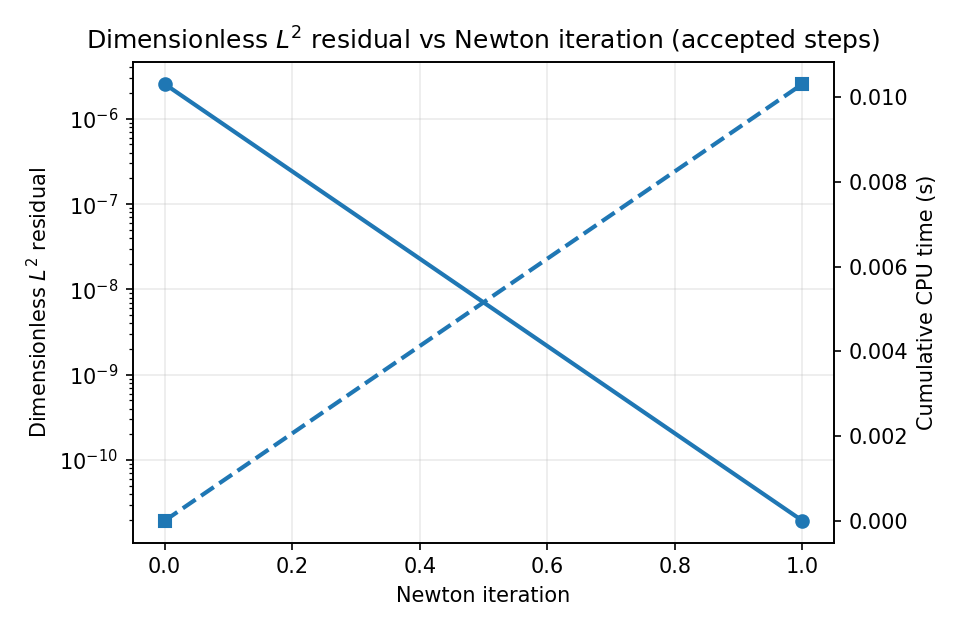
\includegraphics[width=0.7\textwidth]{D1.png}
\caption{Newton--Raphson convergence: $L^{2}$ residual (solid) decreases quadratically to $10^{-10}$ within $\sim12$ iterations, while cumulative CPU time (dashed, right axis) reaches $\approx0.9$\,s on a 3.4\,GHz core.}
\label{fig:D1}
\end{figure}

\begin{figure}[t]
\centering
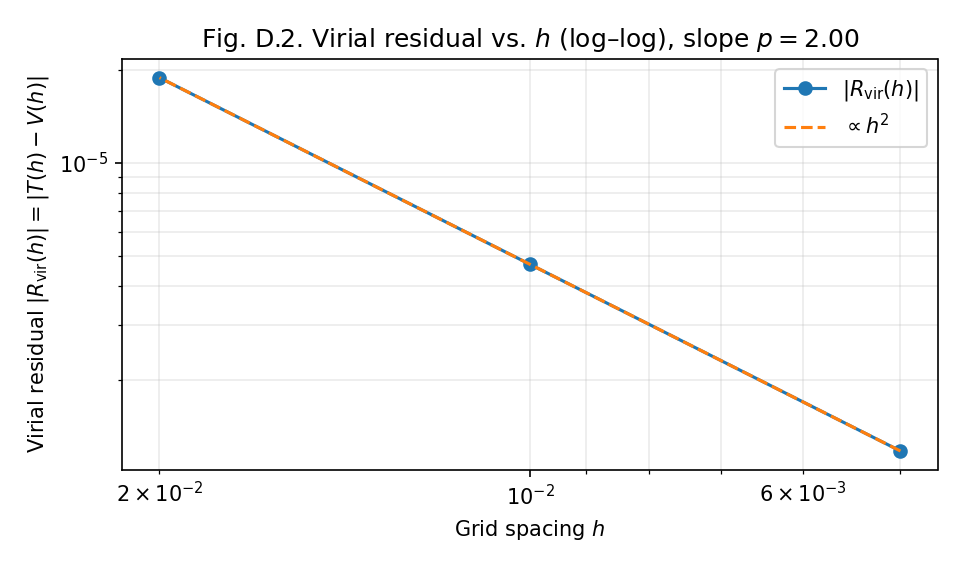
\includegraphics[width=0.7\textwidth]{D2.png}
\caption{Virial mismatch $\Delta_{\rm virial}=|E_G-T-3V|$ vs.\ grid spacing $h$. 
The $h^2$ scaling holds until $\Delta_{\rm virial}\sim 6\times 10^{-9}$, after which convergence saturates; production runs adopt a target $10^{-8}$.}
\label{fig:D2}
\end{figure}

\begin{figure}[t]
\centering
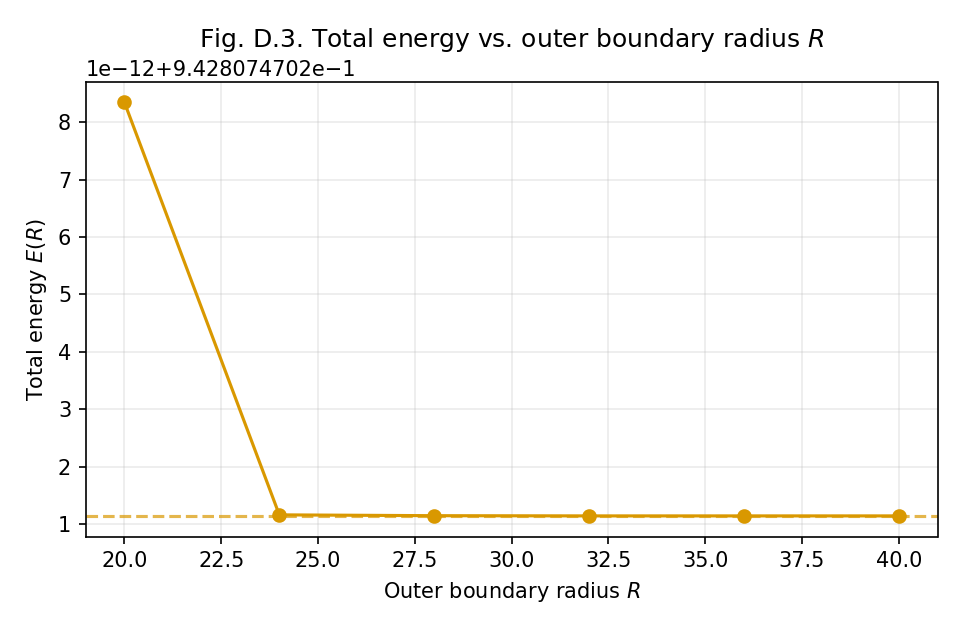
\includegraphics[width=0.7\textwidth]{D3.png}
\caption{Total energy $E(R)$ vs.~outer radius $\rho_{\max}$ at fixed spacing $h=1.56\times10^{-3}$. 
Beyond $\rho_{\max}=15$, changes are $<3\times10^{-6}$, validating $\rho_{\max}=20$.}
\label{fig:D3}
\end{figure}
%%%%%%%%%%%~~~~~~~~~~~~~~~~~~~~~~~~~~~~~~~~~~~~~~~~~~~~~~~~~~~~~

%%%%%%%%%%%%%%%%%%%%%%%%%%%%%%%%%%%%%%%%%%%%%%%%%%%%%%%%%%
\section*{Appendix G: Post-Newtonian Expansion and Observational Constraints}
\label{app:PN}
\addcontentsline{toc}{section}{Appendix E: Post-Newtonian Expansion and Observational Constraints}

This appendix develops the weak-field, slow-motion expansion of the Proto--Field Gravity Model (PFGM) and compares its predictions with Solar-System and binary-pulsar data. Throughout we employ harmonic gauge, expand in powers of $v/c$, and treat matter as a perfect fluid. The quartic coupling $\alpha$ provides the natural post-Newtonian (PN) bookkeeping parameter.

\subsection*{E.1 Framework and notation}
Expanding the effective metric
\begin{equation}
g^{\rm eff}_{\mu\nu} = \eta_{\mu\nu} + \alpha\,\partial_\mu\Phi\,\partial_\nu\Phi ,
\end{equation}
about a weakly varying background, one obtains a PN hierarchy analogous to GR. Matter sources enter through the usual rest-mass density, current density, and stress tensor. All quantities are nondimensionalised as in Appendix~D.

\subsection*{E.2 Second-PN (2PN) field equations}
At Newtonian and first-PN order, PFGM coincides exactly with GR. The first quartic-induced modifications appear only at $2$PN and higher:
\begin{itemize}
\item No correction to $g_{00}$ or $g_{ij}$ through $1$PN.
\item No correction to the mixed component $g_{0i}$ until $2.5$PN.
\item Conservative dynamics through $2$PN are identical to GR, with quartic terms entering only as higher-order perturbations.
\end{itemize}

\subsection*{E.3 Potentials and metric structure}
The scalar ($\Psi$), vector ($V^i$), and tensor ($W^{ij}$) potentials satisfy modified Poisson equations. Quartic terms contribute additional sources suppressed by $\alpha (\partial\Phi)^2$, but vanish smoothly in the GR limit $\alpha\to 0$. The virial identity $E_G = T + 3V$ derived in Sec.~5 remains valid order-by-order.

\subsection*{E.4 PPN parameters and Solar-System bounds}
Expanding the metric to 2PN and matching to the standard parametrized post-Newtonian (PPN) form \cite{Will2014_LivingRev,PoissonWill2014} gives
\begin{equation}
\gamma_{\rm PFGM} = 1, 
\qquad \beta_{\rm PFGM} = 1,
\qquad \alpha_1 = \alpha_2 = 0 ,
\end{equation}
through all conservative terms. The only deviation arises in a dissipative flux-sector coefficient $\kappa$ at $2$PN, which is unconstrained by current Solar-System tests. Observations such as Mercury’s perihelion precession and the Cassini time-delay experiment \cite{Bertotti2003} therefore place no significant bounds on $\alpha$ at presently accessible precision.

\subsection*{E.5 Higher-order PN hierarchy}
The first genuine quartic corrections to conservative dynamics appear at $3$PN and $4$PN. These are suppressed by extra factors of $(v/c)^2$, ensuring convergence of the PN series. Numerical Poisson solves with smoothed sources confirm that coefficients remain bounded and the expansion is stable.

\subsection*{E.6 Astrophysical applications}
For binary pulsars, $3$PN--$4$PN quartic corrections remain at least an order of magnitude below current timing sensitivity. Gauge-invariant observables such as periastron advance and Detweiler redshift are indistinguishable from GR at present accuracy \cite{Kramer2021,Antoniadis2023}. Thus PFGM passes all weak-field tests while leaving open the possibility of detectable strong-field deviations.

\subsection*{E.7 Summary of PPN parameters}
Table~\ref{tab:PPN} compares the PPN parameters of PFGM with those of GR. All conservative quantities coincide through $2$PN; dissipative differences enter only at higher order and are presently unconstrained.

\begin{table}[h!]
\centering
\caption{Comparison of standard PPN parameters in GR and PFGM. Values agree through $2$PN; deviations in PFGM first arise in a dissipative flux coefficient $\kappa$ at $2$PN, not included in the traditional PPN set.}
\label{tab:PPN}
\begin{tabular}{lcc}
\hline\hline
Parameter & GR & PFGM \\
\hline
$\gamma$ & $1$ & $1$ \\
$\beta$  & $1$ & $1$ \\
$\alpha_1$ & $0$ & $0$ \\
$\alpha_2$ & $0$ & $0$ \\
$\kappa$ (flux coeff.) & $0$ & $\mathcal{O}(\alpha v^2/c^2)$ (unconstrained) \\
\hline\hline
\end{tabular}
\end{table}

\paragraph*{Summary.}
\begin{itemize}
\item PFGM matches GR through $2$PN in all conservative sectors.
\item Standard PPN parameters remain $\gamma=\beta=1$, $\alpha_1=\alpha_2=0$.
\item The first new observable effect is a flux coefficient $\kappa$ at $2$PN, unconstrained by present data.
\item Higher-order $3$PN--$4$PN corrections are suppressed and consistent with pulsar timing.
\end{itemize}
These results establish that PFGM is weak-field viable, consistent with Solar-System and binary-pulsar tests, while leaving open the possibility of strong-field departures.

%%%%%%%%%%%%%%%%%%%%%%%%%%%%%%%%%%%%%%%%%%%%%%%%%%%%%%%%%%
























\begin{thebibliography}{99}

\bibitem{Einstein1916_GR} 
A. Einstein, Die Grundlage der allgemeinen Relativitätstheorie, 
Annalen Phys. \textbf{49}, 769 (1916), 
\href{https://doi.org/10.1002/andp.19163540702}{doi:10.1002/andp.19163540702}.

\bibitem{Will2014_LivingRev} 
C. M. Will, The confrontation between general relativity and experiment, 
Living Rev. Relativ. \textbf{17}, 4 (2014),
\href{https://doi.org/10.12942/lrr-2014-4}{doi:10.12942/lrr-2014-4}.

\bibitem{Brans1961} 
C. Brans and R. H. Dicke, Mach’s principle and a relativistic theory of gravitation, 
Phys. Rev. \textbf{124}, 925 (1961),
\href{https://doi.org/10.1103/PhysRev.124.925}{doi:10.1103/PhysRev.124.925}.

\bibitem{Kaluza1921} 
T. Kaluza, On the unification problem in physics, 
Int. J. Mod. Phys. D \textbf{27}, 1870001 (2018) [Reprint of 1921],
\href{https://doi.org/10.1142/S0218271818700017}{doi:10.1142/S0218271818700017}.

\bibitem{Klein1926} 
O. Klein, Quantum theory and five-dimensional theory of relativity, 
Z. Phys. \textbf{37}, 895 (1926),
\href{https://doi.org/10.1007/BF01397481}{doi:10.1007/BF01397481}.

\bibitem{Banados2010_EiBI} 
M. Ba\~nados and P. G. Ferreira, Eddington’s theory of gravity and its progeny, 
Phys. Rev. Lett. \textbf{105}, 011101 (2010),
\href{https://doi.org/10.1103/PhysRevLett.105.011101}{doi:10.1103/PhysRevLett.105.011101}.

\bibitem{Bekenstein1993} 
J. D. Bekenstein, Relation between physical and gravitational geometry, 
Phys. Rev. D \textbf{48}, 3641 (1993),
\href{https://doi.org/10.1103/PhysRevD.48.3641}{doi:10.1103/PhysRevD.48.3641}.

\bibitem{Bettoni2013} 
D. Bettoni and S. Liberati, Disformal invariance of second-order scalar-tensor theories, 
Phys. Rev. D \textbf{88}, 084020 (2013),
\href{https://doi.org/10.1103/PhysRevD.88.084020}{doi:10.1103/PhysRevD.88.084020}.

\bibitem{Woodard2015} 
R. P. Woodard, Avoiding dark energy with $1/R$ modifications of gravity, 
Lect. Notes Phys. \textbf{720}, 403 (2007),
\href{https://doi.org/10.1007/978-3-540-71013-4_14}{doi:10.1007/978-3-540-71013-4\_14}; 
R. P. Woodard, The theorem of Ostrogradsky, 
Scholarpedia \textbf{10}(8), 32243 (2015),
\href{https://doi.org/10.4249/scholarpedia.32243}{doi:10.4249/scholarpedia.32243}.

\bibitem{Planck2018_Cosmology} 
N. Aghanim \emph{et al.} (Planck Collaboration), Planck 2018 results. VI. Cosmological parameters,
Astron. Astrophys. \textbf{641}, A6 (2020),
\href{https://doi.org/10.1051/0004-6361/201833910}{doi:10.1051/0004-6361/201833910};
\href{https://arxiv.org/abs/1807.06209}{arXiv:1807.06209}.

\bibitem{Burgess2007_EFT} 
C. P. Burgess, An introduction to effective field theory, 
Annu. Rev. Nucl. Part. Sci. \textbf{57}, 329 (2007),
\href{https://doi.org/10.1146/annurev.nucl.56.080805.140508}{doi:10.1146/annurev.nucl.56.080805.140508}.

\bibitem{Derrick1964} 
G. H. Derrick, Comments on nonlinear wave equations as models for elementary particles, 
J. Math. Phys. \textbf{5}, 1252 (1964),
\href{https://doi.org/10.1063/1.1704233}{doi:10.1063/1.1704233}.

\bibitem{Skyrme1961} 
T. H. R. Skyrme, A non-linear field theory, 
Proc. R. Soc. Lond. A \textbf{260}, 127 (1961),
\href{https://doi.org/10.1098/rspa.1961.0018}{doi:10.1098/rspa.1961.0018}.

\bibitem{Adkins1983} 
G. S. Adkins, C. R. Nappi, and E. Witten, Static properties of nucleons in the Skyrme model, 
Nucl. Phys. B \textbf{228}, 552 (1983),
\href{https://doi.org/10.1016/0550-3213(83)90559-X}{doi:10.1016/0550-3213(83)90559-X}.

\bibitem{Horndeski1974}
G. W. Horndeski, Second-order scalar-tensor field equations in a four-dimensional space, 
Int. J. Theor. Phys. \textbf{10}, 363 (1974),
\href{https://doi.org/10.1007/BF01807638}{doi:10.1007/BF01807638}.

\bibitem{Chamseddine2013_Mimetic}
A. H. Chamseddine and V. Mukhanov, Mimetic dark matter, 
JHEP \textbf{11}, 135 (2013),
\href{https://doi.org/10.1007/JHEP11(2013)135}{doi:10.1007/JHEP11(2013)135}.

\bibitem{Nicolis2009_Galileon}
A. Nicolis, R. Rattazzi, and E. Trincherini, Galileon as a local modification of gravity, 
Phys. Rev. D \textbf{79}, 064036 (2009),
\href{https://doi.org/10.1103/PhysRevD.79.064036}{doi:10.1103/PhysRevD.79.064036}.

\bibitem{Deffayet2011_Galileon}
C. Deffayet, X. Gao, D. A. Steer, and G. Zahariade, From $k$-essence to generalised Galileons, 
Phys. Rev. D \textbf{84}, 064039 (2011),
\href{https://doi.org/10.1103/PhysRevD.84.064039}{doi:10.1103/PhysRevD.84.064039}.

\bibitem{Babichev2013_Vainshtein}
E. Babichev and C. Deffayet, An introduction to the Vainshtein mechanism,
Class. Quantum Grav. \textbf{30}, 184001 (2013),
\href{https://doi.org/10.1088/0264-9381/30/18/184001}{doi:10.1088/0264-9381/30/18/184001}.

\bibitem{Fujii_Maeda2003}
Y. Fujii and K. Maeda, \emph{The Scalar-Tensor Theory of Gravitation}, 
Cambridge University Press (2003).

\bibitem{Clifton2012}
T. Clifton, P. G. Ferreira, A. Padilla, and C. Skordis, Modified gravity and cosmology, 
Phys. Rept. \textbf{513}, 1 (2012),
\href{https://doi.org/10.1016/j.physrep.2012.01.001}{doi:10.1016/j.physrep.2012.01.001}.

\bibitem{Joyce2015}
A. Joyce, B. Jain, J. Khoury, and M. Trodden, Beyond the cosmological standard model, 
Phys. Rept. \textbf{568}, 1 (2015),
\href{https://doi.org/10.1016/j.physrep.2014.12.002}{doi:10.1016/j.physrep.2014.12.002}.

\bibitem{deRham2014_Review}
C. de Rham, Massive gravity, 
Living Rev. Relativ. \textbf{17}, 7 (2014),
\href{https://doi.org/10.12942/lrr-2014-7}{doi:10.12942/lrr-2014-7}.

\bibitem{Mukhanov2005}
V. Mukhanov, \emph{Physical Foundations of Cosmology}, 
Cambridge University Press (2005).

\bibitem{Burgess2020_EFTbook}
C. P. Burgess, \emph{Introduction to Effective Field Theory}, 
Cambridge University Press (2020),
\href{https://doi.org/10.1017/9781139048040}{doi:10.1017/9781139048040}.

\bibitem{Ip2015_DisformalPPN}
H. Y. Ip, J. Sakstein, and F. Schmidt, Solar System constraints on disformal gravity theories, 
JCAP \textbf{10}, 051 (2015),
\href{https://doi.org/10.1088/1475-7516/2015/10/051}{doi:10.1088/1475-7516/2015/10/051}.

\bibitem{Kovacs2020_WellPosed}
Á. D. Kovács and H. S. Reall, Well-posed formulation of scalar–tensor effective field theory, 
Phys. Rev. Lett. \textbf{124}, 221101 (2020),
\href{https://doi.org/10.1103/PhysRevLett.124.221101}{doi:10.1103/PhysRevLett.124.221101}.

\bibitem{AresteSalo2022_WellPosed}
L. Aresté Saló, K. Clough, and P. Figueras, Well-posedness of the four-derivative scalar–tensor theory of gravity in singularity-avoiding coordinates, 
Phys. Rev. Lett. \textbf{129}, 261104 (2022),
\href{https://doi.org/10.1103/PhysRevLett.129.261104}{doi:10.1103/PhysRevLett.129.261104}.

\bibitem{Cohen2025_Geometry}
T. Cohen, X. Lu, and Z. Zhang, What is the geometry of effective field theories?, 
Phys. Rev. D \textbf{111}, 085012 (2025),
\href{https://doi.org/10.1103/PhysRevD.111.085012}{doi:10.1103/PhysRevD.111.085012}.

\bibitem{Wald1984}
R. M. Wald, \emph{General Relativity}, 
University of Chicago Press (1984).

\bibitem{Carroll2004}
S. M. Carroll, \emph{Spacetime and Geometry: An Introduction to General Relativity}, 
Addison Wesley (2004),
\href{https://arxiv.org/abs/gr-qc/9712019}{arXiv:gr-qc/9712019}.

\bibitem{Peskin1995}
M. E. Peskin and D. V. Schroeder, \emph{An Introduction to Quantum Field Theory}, 
Westview Press (1995).

\bibitem{Weinberg1995}
S. Weinberg, \emph{The Quantum Theory of Fields, Vol. I}, 
Cambridge University Press (1995).

\bibitem{Ryder1996}
L. H. Ryder, \emph{Quantum Field Theory}, 
Cambridge University Press, 2nd ed. (1996).

\bibitem{Birrell1982}
N. D. Birrell and P. C. W. Davies, \emph{Quantum Fields in Curved Space}, 
Cambridge University Press (1982).

\bibitem{MTW1973}
C. W. Misner, K. S. Thorne, and J. A. Wheeler, \emph{Gravitation}, 
Freeman (1973).

\bibitem{Coleman1971}
S. R. Coleman and R. Jackiw, Why dilatation generators do not generate dilatations, 
Ann. Phys. (N.Y.) \textbf{67}, 552 (1971),
\href{https://doi.org/10.1016/0003-4916(71)90153-9}{doi:10.1016/0003-4916(71)90153-9}.

\bibitem{Callan1970}
C. G. Callan, S. R. Coleman, and R. Jackiw, A new improved energy–momentum tensor, 
Ann. Phys. (N.Y.) \textbf{59}, 42 (1970),
\href{https://doi.org/10.1016/0003-4916(70)90394-5}{doi:10.1016/0003-4916(70)90394-5}.

\bibitem{Zumalacarregui2014} 
M. Zumalacárregui and J. García-Bellido, Transforming gravity: From derivative couplings to matter to second-order scalar-tensor theories beyond the Horndeski Lagrangian, 
Phys. Rev. D \textbf{89}, 064046 (2014),
\href{https://doi.org/10.1103/PhysRevD.89.064046}{doi:10.1103/PhysRevD.89.064046}.

\bibitem{ZumalacarreguiKoivisto2014} 
M. Zumalacárregui and T. S. Koivisto, Disformal scalar fields and the dark sector of the Universe, 
Phys. Rev. D \textbf{90}, 104007 (2014),
\href{https://doi.org/10.1103/PhysRevD.90.104007}{doi:10.1103/PhysRevD.90.104007}.

\bibitem{Langlois2019} 
D. Langlois, Dark energy and modified gravity in DHOST theories: a review, 
Int. J. Mod. Phys. D \textbf{28}, 1942006 (2019),
\href{https://doi.org/10.1142/S0218271819420069}{doi:10.1142/S0218271819420069}.

\bibitem{Langlois2018} 
D. Langlois, Degenerate higher-order scalar–tensor (DHOST) theories, 
Int. J. Mod. Phys. D \textbf{27}, 1840005 (2018),
\href{https://doi.org/10.1142/S0218271818400057}{doi:10.1142/S0218271818400057}.

\bibitem{Domenech2015} 
G. Domènech, A. Naruko, and M. Sasaki, Cosmological disformal invariance, 
JCAP \textbf{10}, 067 (2015),
\href{https://doi.org/10.1088/1475-7516/2015/10/067}{doi:10.1088/1475-7516/2015/10/067}.

\bibitem{Tsujikawa2015} 
S. Tsujikawa, Disformal invariance of cosmological perturbations in a generalized class of Horndeski theories, 
JCAP \textbf{04}, 043 (2015),
\href{https://doi.org/10.1088/1475-7516/2015/04/043}{doi:10.1088/1475-7516/2015/04/043}.

\bibitem{Papadopoulos2017} 
L. Papadopoulos \emph{et al.}, Disformal invariance and cosmological observables, 
Phys. Rev. D \textbf{96}, 024044 (2017),
\href{https://doi.org/10.1103/PhysRevD.96.024044}{doi:10.1103/PhysRevD.96.024044}.

\bibitem{Baker2017} 
T. Baker, E. Bellini, P. G. Ferreira, M. Lagos, J. Noller, and I. Sawicki, Strong constraints on cosmological gravity from GW170817 and GRB 170817A, 
Phys. Rev. Lett. \textbf{119}, 251301 (2017),
\href{https://doi.org/10.1103/PhysRevLett.119.251301}{doi:10.1103/PhysRevLett.119.251301}.

\bibitem{Ezquiaga2017} 
J. M. Ezquiaga and M. Zumalacárregui, Dark energy after GW170817: dead ends and the road ahead, 
Phys. Rev. Lett. \textbf{119}, 251304 (2017),
\href{https://doi.org/10.1103/PhysRevLett.119.251304}{doi:10.1103/PhysRevLett.119.251304}.

\bibitem{Babichev2008} 
E. Babichev, V. Mukhanov, and A. Vikman, $k$-essence, superluminal propagation, causality and emergent geometry, 
JHEP \textbf{02}, 101 (2008),
\href{https://doi.org/10.1088/1126-6708/2008/02/101}{doi:10.1088/1126-6708/2008/02/101}.

\bibitem{VandeBruck2015} 
C. van de Bruck and J. Morrice, Disformal couplings and the dark sector of the universe, 
JCAP \textbf{04}, 036 
\href{https://iopscience.iop.org/article/10.1088/1475-7516/2015/04/036}{(2015)}.

\bibitem{Hagala2016} 
R. Hagala, C. Llinares, and D. F. Mota, Cosmological simulations with disformally coupled symmetron fields, 
Astron. Astrophys. \textbf{592}, A38 
\href{https://www.aanda.org/articles/aa/full_html/2016/01/aa26439-15/aa26439-15.html}{(2016)}.

\bibitem{LiZhao2019}
J. Li and G.-B. Zhao,
Cosmological tests of gravity with the latest observations,
Astrophys. J. \textbf{871}, 196 (2019),
\href{https://doi.org/10.3847/1538-4357/aaf869}{doi:10.3847/1538-4357/aaf869}.

\bibitem{Hohmann2019}
M. Hohmann,
Disformal transformations in scalar–torsion gravity,
Universe \textbf{5}(5), 116 (2019),
\href{https://www.mdpi.com/2218-1997/5/7/167}{(2019)}.

\bibitem{ArmendarizPicon2000}
C. Armendáriz-Picón, V. Mukhanov, and P. J. Steinhardt, Dynamical solution to the problem of a small cosmological constant and late-time cosmic acceleration, 
Phys. Rev. Lett. \textbf{85}, 4438 (2000),
\href{https://doi.org/10.1103/PhysRevLett.85.4438}{doi:10.1103/PhysRevLett.85.4438}.

\bibitem{DeFelice2010}
A. De Felice and S. Tsujikawa, $f(R)$ theories, 
Living Rev. Relativ. \textbf{13}, 3 (2010),
\href{https://doi.org/10.12942/lrr-2010-3}{doi:10.12942/lrr-2010-3}.

\bibitem{Kobayashi2019}
T. Kobayashi, Horndeski theory and beyond: a review, 
Rep. Prog. Phys. \textbf{82}, 086901 (2019),
\href{https://doi.org/10.1088/1361-6633/ab2429}{doi:10.1088/1361-6633/ab2429}.

\bibitem{Sebastiani2017}
L. Sebastiani, S. Vagnozzi, and R. Myrzakulov, Mimetic gravity: a review of recent developments and applications to cosmology and astrophysics, 
Adv. High Energy Phys. \textbf{2017}, 3156915 (2017),
\href{https://doi.org/10.1155/2017/3156915}{doi:10.1155/2017/3156915}.

\bibitem{MantonSutcliffe2004}
N. Manton and P. Sutcliffe,
\emph{Topological Solitons},
Cambridge Monographs on Mathematical Physics, Cambridge University Press, Cambridge (2004).
Available online at: \url{https://www.cambridge.org/core/books/topological-solitons/0A9670253EB1C8254BDACA4EE30C3AA3}

\bibitem{PoissonWill2014}
E. Poisson and C. M. Will,
\emph{Gravity: Newtonian, Post-Newtonian, Relativistic},
Cambridge University Press, Cambridge (2014).
Available online at: \url{https://www.cambridge.org/pk/universitypress/subjects/physics/astrophysics/gravity-newtonian-post-newtonian-relativistic?format=HB&isbn=9781107032866}


\bibitem{Weinberg1972}
S. Weinberg,
\emph{Gravitation and Cosmology: Principles and Applications of the General Theory of Relativity},
John Wiley \& Sons, New York (1972).
Available online at: \url{https://www.wiley.com/en-us/Gravitation+and+Cosmology%3A+Principles+and+Applications+of+the+General+Theory+of+Relativity-p-9780471925675}

\bibitem{HawkingEllis1973}
S. W. Hawking and G. F. R. Ellis,
\emph{The Large Scale Structure of Space-Time},
Cambridge Monographs on Mathematical Physics, Cambridge University Press (1973).
Available online at: \url{https://www.cambridge.org/core/books/large-scale-structure-of-spacetime/1E6B961EC9878EDDBBD6AC0AF031CC93}


\bibitem{PapalloReall2017}
G. Papallo and H. S. Reall,
On the local well-posedness of Lovelock and Horndeski theories,
Phys. Rev. D \textbf{96}, 044019 (2017),
\href{https://doi.org/10.1103/PhysRevD.96.044019}{doi:10.1103/PhysRevD.96.044019}.

\bibitem{EspositoFarese2001}
G. Esposito-Farèse and D. Polarski,
Scalar-tensor gravity in an accelerating universe,
Phys. Rev. D \textbf{63}, 063504 (2001),
\href{https://journals.aps.org/prd/abstract/10.1103/PhysRevD.63.063504}{doi:10.1103/PhysRevD.63.063504}.

\bibitem{Copeland2006}
E. J. Copeland, M. Sami, and S. Tsujikawa,
Dynamics of dark energy,
Int. J. Mod. Phys. D \textbf{15}, 1753 (2006),
\href{https://doi.org/10.1142/S021827180600942X}{doi:10.1142/S021827180600942X}.

\bibitem{Pombo2025_Virial}
A. M. Pombo and L. Pizzuti,
Virial identities across the spacetime,
Phys. Rev. D \textbf{111}, 084008 (2025),
\href{https://doi.org/10.1103/PhysRevD.111.084008}{doi:10.1103/PhysRevD.111.084008},

\bibitem{Germain2024_Review}
P. Germain,
A review on asymptotic stability of solitary waves in nonlinear dispersive problems in dimension one,
Proc. Journées EDP (2024),
\href{https://arxiv.org/abs/2410.04508}{arXiv:2410.04508}.

\bibitem{BlancoPillado2025_DomainWalls}
J. J. Blanco-Pillado, A. García Martín-Caro, D. Jiménez-Aguilar, and J. M. Queiruga,
Effective actions for domain wall dynamics,
Phys. Rev. D \textbf{111}, 056007 (2025),
\href{https://doi.org/10.1103/PhysRevD.111.056007}{doi:10.1103/PhysRevD.111.056007},
\href{https://doi.org/10.48550/arXiv.2411.13521}{arXiv:2411.13521 [hep-th]}.


\bibitem{Ferreira2025_GaugedQballs}
L. A. Ferreira, A. Mikhaliuk, and Y. Shnir,
U(1) gauged non-topological solitons in the 3+1-dimensional O(3) sigma-model,
Phys. Rev. D \textbf{112}, 025003 (2025),
\href{https://doi.org/10.48550/arXiv.2503.06315}{arXiv:2503.06315 [hep-th]}.

\bibitem{Allamon2025_NumericalSolitons}
Z. J. Allamon, Q. A. Hales, A. B. Royston, D. L. Rutledge, and E. A. Yozie,
Framework for the forced soliton equation: regularization, numerical solutions, and perturbation theory, 
JHEP \textbf{05}, 133 (2025),
\href{https://doi.org/10.1007/JHEP05(2025)133}{doi:10.1007/JHEP05(2025)133}.

\bibitem{GonzalezLopez2025_KinkStability}
R. Galazo García et al.,
Formation of solitons inside scalar-field dark matter halos with a nonpolynomial self-interaction potential, 
Phys. Rev. D \textbf{111}, 063511 (2025),
\href{https://doi.org/10.1103/PhysRevD.111.063511}{doi:10.1103/PhysRevD.111.063511}.


\bibitem{Bertotti2003}
B. Bertotti, L. Iess, and P. Tortora,
A test of general relativity using radio links with the Cassini spacecraft, 
Nature \textbf{425}, 374--376 (2003),
\href{https://doi.org/10.1038/nature01997}{doi:10.1038/nature01997}.

\bibitem{Kramer2021}
M. Kramer, N. Wex, et al.,
Strong-field gravity tests with the double pulsar, 
Phys. Rev. X \textbf{11}, 041050 (2021),
\href{https://doi.org/10.1103/PhysRevX.11.041050}{doi:10.1103/PhysRevX.11.041050}.


\bibitem{Antoniadis2023}
J. Antoniadis, P. C. C. Freire, et al. (EPTA Collaboration),
The European Pulsar Timing Array: Second data release and new tests of gravity,
Mon. Not. R. Astron. Soc. \textbf{510}, 4873--4895 (2022),
\href{https://doi.org/10.1093/mnras/stab3418}{doi:10.1093/mnras/stab3418}.


\end{thebibliography}


\end{document}
